\documentclass[serif,professionalfont,cjk]{beamer}
\mode<presentation>{
%\usetheme{Warsaw}
%\usetheme{CambridgeUS}
\usetheme{Madrid}
%  \usecolortheme{beaver}
%  \setbeamercovered{transparent}
}
%\usepackage[T1]{fontenc} 
%\usepackage{concrete}
%% \usepackage[T1]{fontenc} % Needed for Type1 Concrete
%% %% \usepackage{concrete} % Loads Concrete + Euler VM
%% %% \usepackage{pxfonts} % Or palatino or mathpazo
%% \usepackage{eulervm} %
%% %% \usepackage{kerkis} % Kerkis roman and sans
%% %% \usepackage{kmath} % Kerkis math
%% \usepackage{fourier}
\usepackage{etex}
\usepackage{pgf}
\usepackage{tikz}
\usetikzlibrary{calc}
\usetikzlibrary{arrows,snakes,backgrounds,shapes,shadows}
\usetikzlibrary{matrix,fit,positioning,decorations.pathmorphing}
\usepackage{CJK} 
\usepackage{amsmath,amssymb,amsfonts}
\usepackage{mathdots}
\usepackage{caption}
\usepackage{verbatim,color,xcolor}
\usepackage{graphicx}
\usepackage{manfnt}
\usepackage{fancybox}
\usepackage{textcomp}
\usepackage{multirow,multicol}
\usepackage{parcolumns}
\usepackage{framed}
\usepackage{threeparttable}
\usepackage{extarrows}
\usepackage{listings}
\lstset{
  keywordstyle=\color{blue!70},
  frame=single,
  basicstyle=\ttfamily\small,
  commentstyle=\small\color{red},
  breakindent=0pt,
  rulesepcolor=\color{red!20!green!20!blue!20},
  rulecolor=\color{black},
  tabsize=4,
  numbersep=5pt,
  breaklines=true,
  %% backgroundcolor=\color{red!10},
  showspaces=false,
  showtabs=false,
  extendedchars=false,
  escapeinside=``,
  frame=no,
}
%% \usepackage[utf8]{inputenc}
%% \usepackage[upright]{fourier}   %


%\usepackage{xcolor}
%\usepackage{pgf}
%\usepackage{tikz}
\usepackage{pgfplots}
%\usetikzlibrary{calc}
%\usetikzlibrary{arrows,snakes,backgrounds,shapes}
%\usetikzlibrary{matrix,fit,positioning,decorations.pathmorphing}
%\usepackage{CJK}               
%\usepackage[italian,american]{babel}
%\usepackage[applemac]{inputenc}
%\usepackage[T1]{fontenc}
%\usepackage{amsmath,amssymb,amsthm}
%\usepackage{varioref}
%\usepackage[style=philosophy-modern,hyperref,square,natbib]{biblatex}
%\usepackage{chngpage}
%\usepackage{calc}
%\usepackage{listings}
%\usepackage{graphicx}
\usepackage{subfigure}
%\usepackage{multicol}
%\usepackage{makeidx}
%\usepackage{fixltx2e}
%\usepackage{relsize}
%\usepackage{lipsum}
\usepackage{xifthen}
%%% \usepackage[eulerchapternumbers,subfig,beramono,eulermath,pdfspacing,listings]{classicthesis}
%%% \usepackage{arsclassica}        
%\usepackage{titlesec} %设置标题
%\usepackage{titletoc}
%\usepackage{extarrows}
%\usepackage{enumerate}

% ######### DEFINE COLOR ###############
\definecolor{blue}{rgb}{0.0,0.0,1.0}
\definecolor{red}{rgb}{1.0,0.0,0.0}
\definecolor{purple}{rgb}{0.75, 0.0, 1.0}


%%%% \renewcommand *****
%\renewcommand{\lstlistingname}{}
%\newcommand{\tf}{\ttfamily}
%\newcommand{\ttt}{\texttt}
%\newcommand{\blue}{\textcolor{blue}}
%\newcommand{\red}{\textcolor{red}}
%\newcommand{\purple}{\textcolor{purple}}
\newcommand{\ft}{\frametitle}
\newcommand{\fst}{\framesubtitle}
\newcommand{\bs}{\boldsymbol}
\newcommand{\ds}{\displaystyle}
\newcommand{\vd}{\vdots}
\newcommand{\cd}{\cdots}
\newcommand{\dd}{\ddots}
\newcommand{\id}{\iddots}
\newcommand{\XX}{\mathbf{X}}
\newcommand{\PP}{\mathbf{P}}
\newcommand{\QQ}{\mathbf{Q}}
\newcommand{\xx}{\mathbf{x}}
\newcommand{\yy}{\mathbf{y}}
\newcommand{\bb}{\mathbf{b}}
\newcommand{\abd}{\boldsymbol{a}}
%\newcommand{\A}{\mathbf{A}}
%\newcommand{\B}{\mathbf{B}}
%\newcommand{\C}{\mathbf{C}}
%\newcommand{\D}{\mathbf{D}}
%\newcommand{\E}{\mathbf{E}}
%\newcommand{\X}{\mathbf{X}}
%\newcommand{\Y}{\mathbf{Y}}
%\newcommand{\Z}{\mathbf{Z}}
\newcommand{\R}{\mathbb{R}}
%\newcommand{\T}{\mathbf{T}}
%\newcommand{\zero}{\mathbf{0}}
%\newcommand{\II}{\mathbf{I}}
%\newcommand{\LLambda}{\mathbf{\Lambda}}
%\newcommand{\alphabd}{\boldsymbol{\alpha}}
%\newcommand{\betabd}{\boldsymbol{\beta}}
%\newcommand{\gammabd}{\boldsymbol{\gamma}}
%
%\newcommand{\Loc}{\mathrm{Loc}}



\begin{document}
\begin{CJK}{UTF8}{gkai} 
\CJKtilde
\renewcommand{\proofname}{\vspace{0.2cm}\textbf{证明: \ }}
\newcommand{\jiename}{\vspace{0.2cm}\textbf{解: \ }}

\renewcommand{\figurename}{图}  

\renewcommand{\proofname}{证明}
\newtheorem*{jie}{解}
\newtheorem*{zhu}{注}
\newtheorem{dingli}{定理} 
\newtheorem{dingyi}{定义} 
\newtheorem{li}{例} 


\title{数据结构与算法}
\subtitle{线性表}
\institute[]{
  
\includegraphics[width=0.5in]{wuda_log.pdf} \\
  数学与统计学院 \\
  Email: ~~ xpzhang.math@whu.edu.cn    \\
  Homepage: ~~http://staff.whu.edu.cn/show.jsp?n=Zhang\%20Xiaoping
}

\author{张晓平}
\date{}
\subject{数据结构与算法}
% 如果你想插入学校的徽章, 其文件名为 "university-logo-filename.xxx", 
% 其中 xxx 是 pdflatex 能接受的格式, 则可用以下命令插入
%% \pgfdeclareimage[height=0.5cm]{wuda}{wudalogo.pdf}
%% \logo{\pgfuseimage{wuda}}
%% \pgfdeclareimage[width=1.0cm]{university-logo}{university-logo-filename.jpg}
%% \logo{\pgfuseimage{university-logo}}

% 如果你想要在每一小节之前都显示一下目录, 则可把一下小段的注解号 "%" 删去
%% \AtBeginSubsection[]
%% {
%%  \begin{frame}<beamer>
%%    \frametitle{概要}
%%    \tableofcontents[currentsection,currentsubsection]
%%  \end{frame}
%% }

%除掉以下命令的注解 "%" 后, 许多环境都会自动逐段显示
% \beamerdefaultoverlayspecification{<+->}

%% 的演示文稿仅供参考, 不过可以提供一些忠告:
% - 除总结外, 最好不超过 3 节;
% - 每节至多分成 3 小节;
% - 每屏约 30 秒至 2 分钟, 因此总共 15 至 30 屏为佳.
% - 一般说来, 会议听众对你所报告的东西知之甚少, 因此尽量简单!
% - 在 20 分钟报告里只要讲清主要思想即可, 不要深入细节, 宁可牺牲一点严格性;
% - 如果你略去了证明或实现的关键细节, 只要声明一下即可, 没有人会感到不高兴.





\begin{frame}
\titlepage
\end{frame}

\begin{frame}
\frametitle{目录}
\tableofcontents[subsectionstyle=hide]
\end{frame}

\AtBeginSection[]{
\begin{frame}[allowframebreaks]
\tableofcontents[currentsection,hideallsubsections]
\end{frame}
}
\AtBeginSubsection[]{
\begin{frame}[allowframebreaks]
\tableofcontents[currentsection,sectionstyle=show/shaded]%,subsectionstyle=show/shaded/hide]
\end{frame}
}

%  \begin{frame}
    \begin{figure}
      \centering
      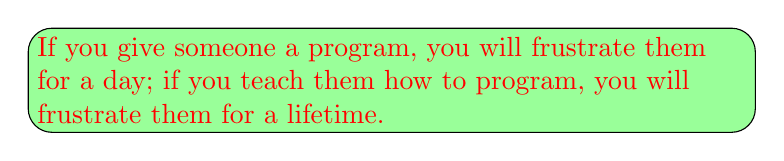
\begin{tikzpicture}
        \node [rectangle,fill=green!40,draw,rounded corners=3mm,text width=9cm,text=red] {
          If you give someone a program, you will frustrate them for a day; 
          if you teach them how to program, you will frustrate them for a lifetime.
        };
      \end{tikzpicture}    
    \end{figure}
  \end{frame}

  \begin{frame}
    \begin{figure}
      \centering
      
\includegraphics[width=2in]{Chapters/Ch01/Fig/DsAlgYan}
      \caption{参考用书}
    \end{figure}
  \end{frame}


\section{数值计算简介}

%%%%%%%%%%%%%%%%%
\begin{frame}\frametitle{\secname} %\fst{现代科学的三大手段}
当今世界科学活动的三种主要方式\\

\begin{itemize}
\item
理论
\item
实验
\item
科学计算
\end{itemize}
\end{frame}
%
%%%%%%%%%%%%%%%%%%
\tikzstyle{decision} = [diamond, draw, fill=blue!20,
text width=4.5em, text badly centered, node distance=3cm, inner sep=0pt]
\tikzstyle{block} = [rectangle, draw, fill=blue!20,
text width=2em, text centered, rounded corners, minimum height=4em]
\tikzstyle{line} = [draw, -latex']
\begin{frame}\ft{\secname}%\fst{解决科学工程问题的步骤}
\begin{figure}
\centering
\begin{tikzpicture}[scale=0.5, node distance = 2.0cm, auto]
  \pause
  \node [block] (problem) {实\\ 际\\ 问\\ 题};

  \pause

  \node [block, right of=problem] (model) {数\\ 学\\ 模\\ 型};
  \path [line] (problem) -- (model);
  \pause

  \node [block, right of=model] (method) {计\\算\\方\\法};
  \path [line] (model) -- (method);
  \pause

  \node [block, right of=method] (prog) {程\\ 序\\ 设\\ 计};
  \path [line] (method) -- (prog);
  \pause

  \node [block, right of=prog] (comp) {上\\ 机\\ 求\\ 解};
  \path [line] (prog) -- (comp);
  \pause

  \draw[decorate, decoration={brace, mirror}, very thick, blue] (0,-3.5) -- (4,-3.5);
  \draw (2,-4.5) node {应用数学};
  \pause

  \draw[decorate, decoration={brace, mirror}, very thick, blue] (8,-3.5) -- (16,-3.5);
  \draw (12,-4.5) node {计算数学};
\end{tikzpicture}
\caption{解决科学工程问题的步骤}
\end{figure}
\end{frame}
%
%%%%%%%%%%%%%%%%%
\begin{frame}\ft{\secname}\fst{研究数值方法的必要性}

\begin{li}
  求解线性方程组
  $$
  Ax = b, \quad A \in \R^{n\times n}, \quad b \in \R^n
  $$
\end{li}
\pause
\begin{dingli}[Crammer法则]
  $$
  A\mbox{非奇异}
  ~~\Longrightarrow~~
  \mbox{此方程组有唯一解,且}
  x_i = \frac{|A_i|}{|A|}, ~~ i = 1, \cd, n.
  $$
\end{dingli}

\pause
该结论非常漂亮,它把线性方程组的求解问题归结为计算$n+1$个$n$阶行列式的计算问题。

\end{frame}
%
%%%%%%%%%%%%%%%%%
\begin{frame}\ft{\secname}\fst{研究数值方法的必要性}

对于行列式的计算
\begin{dingli}[Laplace展开定理]
  $$
  |A| = a_{i1} A_{i1} + a_{i2} A_{i2} +  \cd + a_{in} A_{in}, \quad
  A_{ij}\mbox{为}a_{ij}\mbox{的代数余子式}
  $$      
\end{dingli}

\pause
该方法的运算量大的惊人,以至于完全不能用于实际计算。

\end{frame}
%
%%%%%%%%%%%%%%%%%
\begin{frame}\ft{\secname}

设$k$阶行列式所需乘法运算的次数为$m_k$,则
$$
m_k = k + k m_{k-1},
$$
于是有
$$
\begin{array}{ll}
  &m_n = n + n m_{n-1} \\[0.2cm]
  &= n + n[(n-1) + (n-1) m_{n-2}] \\[0.2cm]
  &= \cd \\[0.2cm]
  &= n + n(n-1) + n(n-1)(n-2) + \cd + n(n-1)\cd 3 \cdot 2\\[0.2cm]
  &> n!
\end{array}
$$

\end{frame}
%
%%%%%%%%%%%%%%%%%
\begin{frame}\ft{\secname}

  故用Crammer法则和Laplace展开定理求解一个$n$阶线性方程组,所需乘法运算的次数就大于
$$
(n+1)n! = (n+1)!.
$$

\end{frame}
%
%%%%%%%%%%%%%%%%%
\begin{frame}\ft{\secname}
在一台百亿次的计算机上求解一个25阶线性方程组,则至少需要
$$
\frac{26!}{10^{10}\times 3600 \times 24 \times 365}
\approx
\frac{4.0329\times 10^{28}}{3.1526\times 10^{17}}
\approx
13\mbox{亿年}
$$
\pause
而用下章介绍的消去法求解,则需要不到一秒钟。
\end{frame}
%
%
%
%%%%%%%%%%%%%%%%%
\begin{frame}\ft{\secname}%\fst{研究对象}
数值分析的研究对象为: 
\begin{itemize}
\item
线性代数\\
\item
曲线拟合\\
\item
数值逼近\\
\item
微积分\\
\item
微分方程\\
\item
积分方程\\
\item
$\cdots$
\end{itemize}
\end{frame}

%%%%%%%%%%%%%%%%%
\begin{frame}\ft{\secname}%\fst{研究任务}
数值分析的研究任务为: 
\begin{itemize}
\item
算法设计 
\item
理论分析
\item[]
\begin{itemize}
\item 算法的收敛性 
\item 稳定性 
\item 误差分析
\end{itemize} 

\item
复杂度分析
\item[]
\begin{itemize}
\item 时间复杂度 
\item 空间复杂度
\end{itemize} 
\end{itemize}

\end{frame}
%
%%%%%%%%%%%%%%%%%
\begin{frame}\ft{\secname}%\fst{特点}
数值分析的特点为: 
\begin{itemize}
\item
既有数学的抽象性与严格性,又有广泛的应用性;
\item
有自身的研究方法和理论系统;
\item
与计算机紧密结合,实用性很强。
\end{itemize}

\end{frame}

\section{数值线性代数}

%%%%%%
\begin{frame}\ft{\secname}%\fst{三大基本问题}
\begin{small}

数值线性代数研究的三大基本问题为:\vspace{0.1in}

\begin{block}{一、求解线性方程组}
给定非奇异矩阵$A\in\R^{n\times n}$和向量$b\in\R^n$,求向量$x\in\R^n$使得
$$
Ax = b.
$$
\end{block}
\end{small}
\end{frame}

\begin{frame}\ft{\secname}
\begin{small}
\begin{block}{二、线性最小二乘问题}
给定矩阵$A\in\R^{m\times n}$和向量$b\in\R^n$,求向量$x\in\R^m$使得
$$
\|Ax - b\|_2 = \min \{\|Ax - b\|_2:~ y \in \R^n \}.
$$
\end{block}
\end{small}
\end{frame}

\begin{frame}\ft{\secname} 
\begin{small}
\begin{block}{三、特征值问题}
给定方阵$A\in\R^{n\times n}$,求其特征值(部分或全部)以及对应的特征向量。
\end{block}
\end{small}
\end{frame}


%%%%%%
\begin{frame}\ft{\secname}%\fst{其他问题}
\begin{small}
数值线性代数所研究的其他问题还有:
\begin{itemize}
\item
约束最小二乘问题
\item
完全最小二乘问题
\item
矩阵方程的求解问题
\item
矩阵函数的计算问题
\item
广义特征值问题
%\item
%非线性特征值问题
\item
特征值反问题
\item
\colorbox{fcolor5}{奇异值分解的计算问题}
\end{itemize}
\end{small}
\end{frame}

\section{逻辑结构和物理结构}

\subsection{逻辑结构}
\begin{frame}
  \documentclass{article}
\usepackage{CJK} 
\usepackage{graphics}
\usepackage{pgf}
\usepackage{tikz}
\usetikzlibrary{calc,shadows}
\usetikzlibrary{decorations.markings,scopes}
\usetikzlibrary{arrows,snakes,backgrounds,shapes}
\usetikzlibrary{decorations.pathmorphing}
\newcommand{\blue}{\textcolor{blue}}
\newcommand{\red}{\textcolor{red}}
\newcommand{\purple}{\textcolor{purple}}


\pgfrealjobname{survey}
\begin{document}
\begin{CJK}{UTF8}{gkai} 
  \beginpgfgraphicnamed{LogicStruct}
  \begin{tikzpicture}[scale=2,cap=round]

    % The graphic
    \node at (0,0)[fill=blue!20,draw,starburst,drop shadow,text width=4.5cm]
    {
      \blue{\large 逻辑结构}: 指数据结构中数据元素之间的相互关系.
    } ;

    \node at (0,-1.6) [text width=2.3cm,decorate,decoration=saw,fill=blue!20,draw,circle]
          {
            \begin{itemize}
            \item 集合结构
            \item 线性结构
            \item 树形结构
            \item 图形结构
            \end{itemize}
          };

  \end{tikzpicture}
  \endpgfgraphicnamed  
\end{CJK}

\end{document}

\end{frame}

\begin{frame}
  \documentclass{article}
\usepackage{CJK} 
\usepackage{graphics}
\usepackage{pgf}
\usepackage{tikz}
\usetikzlibrary{calc,shadows}
\usetikzlibrary{decorations.markings,scopes}
\usetikzlibrary{arrows,snakes,backgrounds,shapes}
\usetikzlibrary{decorations.pathmorphing}
\newcommand{\blue}{\textcolor{blue}}
\newcommand{\red}{\textcolor{red}}
\newcommand{\purple}{\textcolor{purple}}


\pgfrealjobname{survey}
\begin{document}
\begin{CJK}{UTF8}{gkai} 
  \beginpgfgraphicnamed{SetStruct}
  
  \begin{tikzpicture}[scale=2,cap=round]

    % The graphic
    \node at (0,2)[fill=blue!20,draw,starburst,drop shadow,text width=6cm]
    {
      \blue{\large 集合结构}: 其中的元素除了同属于一个集合外,之间没有其他关系.
    } ;
    
    \draw (0,0)circle(1);
    \draw (0.00,0.00)node[]{1}circle(0.15);
    \draw (0.55,0.50)node[]{2}circle(0.15);
    \draw (-.65,-.10)node[]{3}circle(0.15);
    \draw (-.35,0.30)node[]{4}circle(0.15);
    \draw (0.80,0.10)node[]{5}circle(0.15);
    \draw (0.25,-.70)node[]{6}circle(0.15);
    \draw (-.15,0.70)node[]{7}circle(0.15);
    \draw (-.45,-.50)node[]{8}circle(0.15);
    \draw (0.55,-.20)node[]{9}circle(0.15);
  \end{tikzpicture}
  \endpgfgraphicnamed  
\end{CJK}

\end{document}

\end{frame}

\begin{frame}
  \begin{figure}  
  \centering
  \begin{tikzpicture}
    \tikzstyle{state}=[draw,circle]

        % The graphic
    \node at (-.5,2)[left,fill=blue!20,draw,starburst,drop shadow,text=red,text centered]
    (1){
      {线性结构}
    } ;
    \node at (.5,2)[right,fill=blue!20,draw,rectangle,rounded corners=3mm,text=blue,text width=7cm]
    (2){
      其中的数据元素之间是一对一的关系.
    }; 
    \pause    
    \node at (0,0) [state] (1) {1};
    \node[state] (2) [right of=1] {2};
    \node[state] (3) [right of=2] {3};
    \node[state] (4) [right of=3] {4};
    \node[state] (5) [right of=4] {5};
    \node[state] (6) [below of=5] {6};
    \node[state] (7) [below of=6] {7};
    \node[state] (8) [left  of=7] {8};
    \node[state] (9) [left  of=8] {9};
    \path 
    (1) edge (2)
    (2) edge (3)
    (3) edge (4)
    (4) edge (5)
    (5) edge (6)
    (6) edge (7)
    (7) edge (8)
    (8) edge (9);
  \end{tikzpicture}
\end{figure}

\end{frame}

\begin{frame}
  \begin{figure}  
  \centering
  \begin{tikzpicture}[level distance=1.5cm,
    level 1/.style={sibling distance=3cm},
    level 2/.style={sibling distance=1.5cm},
    ]
    \tikzstyle{state}=[draw,circle]
        % The graphic
    \node at (-.5,2)[left,fill=blue!20,draw,starburst,drop shadow,text=red,text centered]
    (1){
      {树形结构}
    } ;
    \node at (0.5,2)[right,fill=blue!20,draw,rectangle,rounded corners=3mm,text=blue,text width=6cm]
    (2){
      其中的数据元素之间是一对多的层次关系.
    };
    \pause
    
    \node[state]{A}
    child {node[state]{B}     
      child {node[state]{E}}
      child {node[state]{F}}
      child {node[state]{G}}
    }
    child {node[state]{C}
      child {node[state]{H}}
    }
    child {node[state]{D}     
      child {node[state]{I}}
      child {node[state]{J}}
    };
    
  \end{tikzpicture}
\end{figure}

\end{frame}

\begin{frame}
  \begin{figure}  
  \centering
  \begin{tikzpicture}[scale=1.5]
    \tikzstyle{state}=[draw,circle]

        % The graphic
    \node at (-.5,1.5)[left,fill=blue!20,draw,starburst,drop shadow,text=red,text centered]
    (1){
      {图形结构}
    } ;
    \node at (0.5,1.5)[right,fill=blue!20,draw,rectangle,rounded corners=3mm,text=blue,text width=6.5cm]
    (2){
      其中的数据元素之间是多对多的关系.
    };
    \pause
    \node at (0,0) [state] (1) {1};
    \node at (-1,-0.5) [state] (2)  {2};
    \node at (1.2,-0.5)[state] (3)  {3};
    \node at (-1.5,-1.5)[state] (4)  {4};
    \node at (0.2,-0.8)[state] (5)  {5};
    \node at (0.8,-2.0)[state] (7)  {7};
    \node at (1.8,-2.5)[state] (6)  {6};
    \node at (-0.5,-1.4)[state] (8)  {8};
    \node at (0.1,-2.8)[state] (9)  {9};
    \path 
    (1) edge (2) edge (3)
    (2) edge (4) edge (8) edge (5)
    (3) edge (5) edge (6)
    (4) edge (8) edge (9)
    (5) edge (7) edge (9)
    (6) edge (9)
    (7) edge (6) edge (9)
    (8) edge (9);
  \end{tikzpicture}
\end{figure}

\end{frame}

\begin{frame}
  在用示意图表示数据的逻辑结构时,请注意: \vspace{0.1in}
  
  \begin{itemize}
  \item 将每一个数据元素看做一个结点,用圆圈表示;\\[0.1in]
  \item 元素之间的逻辑关系用结点之间的连线表示,如果这个关系是有方向的,那么用带箭头的连线表示。
  \end{itemize}
  \pause

  \begin{figure}    
    \centering
    \begin{tikzpicture}
      \node [fill=red!20,starburst,drop shadow,draw,text width=7.5cm,text=blue]{
        逻辑结构是针对具体问题的,是为了解决某个问题。在对问题理解的基础上,选择一个合适的数据结构表示数据元素之间的逻辑关系。      
      };
    \end{tikzpicture}

  \end{figure}

\end{frame}


\subsection{物理结构}

\begin{frame}
  
  \documentclass{article}
\usepackage{CJK} 
\usepackage{graphics}
\usepackage{pgf}
\usepackage{tikz}
\usetikzlibrary{calc,shadows}
\usetikzlibrary{decorations.markings,scopes}
\usetikzlibrary{arrows,snakes,backgrounds,shapes}
\usetikzlibrary{decorations.pathmorphing}
\newcommand{\blue}{\textcolor{blue}}
\newcommand{\red}{\textcolor{red}}
\newcommand{\purple}{\textcolor{purple}}


\pgfrealjobname{survey}
\begin{document}
\begin{CJK}{UTF8}{gkai} 
  \beginpgfgraphicnamed{PhyStruct}
  \begin{tikzpicture}[scale=1.5]
    \tikzstyle{state}=[draw,circle]

        % The graphic
    \node at (0,0)[fill=blue!20,draw,starburst,drop shadow,text width=6.5cm]{
      \blue{\large 物理结构}: 指数据的逻辑结构在计算机中的存储方式.
    } ;

    \node at (-1,-2) [fill=blue!20,draw,ellipse callout, callout relative pointer={(0.,0.7)},text width=5.5cm]{ 
      数据的存储结构应正确反映数据元素之间的逻辑关系。如何存储数据元素之间的逻辑关系,是实现物理结构的重点和难点。
    };

    \node at (2.5,-1.3) [text width=1.5cm,decorate,decoration=saw,fill=blue!20,draw,circle,text=red]{
      顺序存储 链式存储
    };

    
  \end{tikzpicture}
  \endpgfgraphicnamed  
\end{CJK}

\end{document}



  
\end{frame}

\begin{frame}
  
  \documentclass{article}
\usepackage{CJK} 
\usepackage{graphics}
\usepackage{pgf}
\usepackage{tikz}
\usetikzlibrary{calc,shadows}
\usetikzlibrary{decorations.markings,scopes}
\usetikzlibrary{arrows,snakes,backgrounds,shapes}
\usetikzlibrary{decorations.pathmorphing}
\newcommand{\blue}{\textcolor{blue}}
\newcommand{\red}{\textcolor{red}}
\newcommand{\purple}{\textcolor{purple}}


\pgfrealjobname{survey}
\begin{document}
\begin{CJK}{UTF8}{gkai} 
  \beginpgfgraphicnamed{SeqStruct}
  \begin{tikzpicture}[scale=1.5]
    \tikzstyle{state}=[draw,circle]

        % The graphic
    \node at (0,2)[right,fill=blue!20,draw,starburst,drop shadow,text width=6.5cm]{
      \blue{\large 顺序存储结构} \\
      把数据元素存放在连续的存储单元里,其数据间的逻辑关系与物理关系一致。
    } ;

    %% \node at (-1,-2) [fill=blue!20,draw,ellipse callout, callout relative pointer={(0.,0.7)},text width=5.5cm]{ 
    %%   数据的存储结构应正确反映数据元素之间的逻辑关系。如何存储数据元素之间的逻辑关系,是实现物理结构的重点和难点。
    %% };

    %% \node at (2.5,-1.3) [text width=1.5cm,decorate,decoration=saw,fill=blue!20,draw,circle,text=red]{
    %%   顺序存储 链式存储
    %% };
    \def\xx{0.8}
    \draw[very thick] (0,0)--(9*\xx,0);
    \foreach \i in {0,...,9} 
    \draw[very thick] (\i*\xx,0)--(\i*\xx,1*\xx);      
    \foreach \i in {1,...,9} 
    \draw[thick] (\i*\xx-0.5*\xx,0.5*\xx)node[]{\i}circle(0.5*\xx);

    
  \end{tikzpicture}
  \endpgfgraphicnamed  
\end{CJK}

\end{document}



  
\end{frame}

\begin{frame}
  
  \documentclass{article}
\usepackage{CJK} 
\usepackage{graphics}
\usepackage{pgf}
\usepackage{tikz}
\usetikzlibrary{calc,shadows}
\usetikzlibrary{decorations.markings,scopes}
\usetikzlibrary{arrows,snakes,backgrounds,shapes}
\usetikzlibrary{decorations.pathmorphing}
\newcommand{\blue}{\textcolor{blue}}
\newcommand{\red}{\textcolor{red}}
\newcommand{\purple}{\textcolor{purple}}


\pgfrealjobname{survey}
\begin{document}
\begin{CJK}{UTF8}{gkai} 
  \beginpgfgraphicnamed{LinkStruct}
  \begin{tikzpicture}[->,>=stealth,scale=1.5]
    \tikzstyle{state}=[draw,circle]

        % The graphic
    \node at (0,2)[right,fill=blue!20,draw,starburst,drop shadow,text width=6.5cm]{
      \blue{\large 链式存储结构} \\
      把数据元素存放在任意的存储单元里,这组存储单元可以连续,也可以不连续。
    } ;

    \node at (5,-1) [fill=blue!20,draw,ellipse callout, callout relative pointer={(0.,0.7)},text width=4cm]{ 
      数据元素的存储关系并不能反映其逻辑关系,需要用一个指针存放数据元素的地址,这样就可以通过地址找到相关联数据元素的位置。
    };

    
    \node at (0,0)    [state] (1) {1};
    \node at (2.3,-0.3) [state] (2)  {2};
    \node at (2.7,0.1) [state] (9)  {9};
    \node at (1.6,-0.6) [state] (3)  {3};
    \node at (1.0,-1.2) [state] (5)  {5};
    \node at (0.0,-1.8) [state] (8)  {8};
    \node at (1.3,-2.5) [state] (6)  {6};
    \node at (2.4,-2.3) [state] (4)  {4};
    \node at (2.6,-1.0) [state] (7)  {7};
    
    \path (1) edge [bend left] (2)
    (2) edge [bend right] (3)
    (3) edge [bend left] (4)
    (4) edge [bend left] (5)
    (5) edge [bend right] (6)
    (6) edge [bend right] (7)
    (7) edge [bend left] (8)
    (8) edge [bend left] (9)
    ;
    
  \end{tikzpicture}
  \endpgfgraphicnamed  
\end{CJK}

\end{document}



  
\end{frame}

\begin{frame}
  
  \documentclass{article}
\usepackage{CJK} 
\usepackage{graphics}
\usepackage{pgf}
\usepackage{tikz}
\usetikzlibrary{calc,shadows}
\usetikzlibrary{decorations.markings,scopes}
\usetikzlibrary{arrows,snakes,backgrounds,shapes}
\usetikzlibrary{decorations.pathmorphing}
\newcommand{\blue}{\textcolor{blue}}
\newcommand{\red}{\textcolor{red}}
\newcommand{\purple}{\textcolor{purple}}


\pgfrealjobname{survey}
\begin{document}
\begin{CJK}{UTF8}{gkai} 
  \beginpgfgraphicnamed{LogicPhySummary}
  \begin{tikzpicture}
  \node[copy shadow,fill=blue!20,draw=blue,thick,text width=7cm] at (3.5,0) {
    逻辑结构是面向问题的,而物理结构是面向计算机的,我们的目标是将数据及其逻辑关系存储到计算机的内存中。
  };
\end{tikzpicture}
  \endpgfgraphicnamed  
\end{CJK}

\end{document}



  
\end{frame}

\section{选用和设计算法应遵循的原则}

%******
\begin{frame}\ft{原则1:数值稳定} 

\begin{flushleft}
一、选用{数值稳定}的计算公式,控制舍入误差的传播
\end{flushleft}
若算法不稳定,则数值计算的结果就会严重背离数学模型的真实结果。
因此在选择数值计算公式来进行近似计算时,应特别注意选用那些在计算过程中不会导致误差迅速增长的计算公式。
\end{frame}

%******
\begin{frame}\ft{原则1:数值稳定} 
\begin{li}
计算积分
$$
I_n = e^{-1} \int_0^1 x^n e^x \,dx, ~~~ n = 0, 1, 2, \cdots
$$
\end{li}
\pause
$$
\textcolor{acolor2}{
\mbox{(算法1)}~\cd\cd~
\left\{
\begin{array}{l}
I_n = 1 - n I_{n-1}, \\[0.3cm]
I_0 = 1 - e^{-1} \approx 0.6321.
\end{array}
\right.
}
$$
\end{frame}


%%******
\begin{frame}[fragile]\ft{原则1:数值稳定} 
\begin{lstlisting}[language=matlab,title=matlab code,frame=single,backgroundcolor=\color{red!10}]
t0 = 0.6321;
for i = 1:9
    fprintf('%10.5f ', t0);
    if(mod(i, 3)==0)
        fprintf('\n');
    end
t1 = 1 - i * t0;
t0 = t1;  
end
\end{lstlisting}
\end{frame}


%%******
\begin{frame}[fragile]\ft{原则1:数值稳定}  
\begin{lstlisting}[title=running result,frame=single,backgroundcolor=\color{blue!10}]
0.63210    0.36790    0.26420 
0.20740    0.17040    0.14800 
0.11200    0.21600   -0.72800 
\end{lstlisting}

 
\end{frame}


\begin{frame}\ft{原则1:数值稳定}  
由
$$
0 < I_n < e^{-1} \max_{0\le x \le 1} (e^x) \int_0^1 x^n \,dx = \frac1{n+1}
$$
知
$$
I_7 < \frac1{8} = 0.1250,
~~~ I_8 < \frac1{9} \approx 0.1111,
$$
\pause
\begin{block}{原因}
$I_0$本身有不超过$0.5\times10^{-4}$的舍入误差,
此误差在运算中传播、积累很快,传播到$I_7$和$I_8$时,该误差已放大了7与8倍,从而使得$I_7$和$I_8$的结果面目全非。
\end{block}
\end{frame}

%******
\begin{frame}\ft{原则1:数值稳定}


$$
\textcolor{acolor2}{\mbox{(算法2)}~\cd\cd~~ I_{n-1} = \frac1n(1-I_n)}
$$


\pause 
由
$$
I_n > e^{-1} \min_{0\le x \le 1} (e^x) \int_0^1 x^n \,dx = \frac{e^{-1}}{n+1}
$$
知
$$
\frac{e^{-1}}{n+1} < I_n < \frac1{n+1}.
$$

$$
I_7 \approx 0.1124.
$$

 
\end{frame}


%******
\begin{frame}[fragile]\ft{原则1:数值稳定}

\begin{lstlisting}[language=matlab,title=matlab code,frame=single,backgroundcolor=\color{red!10}]
t0 = 0.1124;
for i = 7:-1:0
    fprintf('%10.5f ', t0);
    if(mod(7-i+1, 3)==0)
        fprintf('\n');
    end
t1 = (1 - t0) / i;
t0 = t1;    
end
\end{lstlisting}
\end{frame}


%******
\begin{frame}[fragile]\ft{原则1:数值稳定} 
\begin{lstlisting}[title=running result,frame=single,backgroundcolor=\color{blue!10}]
0.11240    0.12680    0.14553 
0.17089    0.20728    0.26424 
0.36788    0.63212 
\end{lstlisting}

 
\end{frame}
%
%
%*****
\begin{frame}\ft{原则1:数值稳定}

\begin{dingyi}[数值稳定]
在数值计算中,误差不会增长的计算格式称为是\textcolor{acolor5}{数值稳定}的,否则就是不稳定的。
\end{dingyi}
 
\end{frame}
%
%
%******
\begin{frame}\ft{原则2:简化计算步骤} 

\begin{flushleft}
二、尽量简化计算步骤,以便减少运算次数
\end{flushleft}
\pause 
节省计算量,提高计算速度,简化逻辑结构,减少误差积累。

 
\end{frame}


%******
\begin{frame}\ft{原则2:简化计算步骤}

\begin{li}
计算多项式
$$
P_n(x) = a_n x^n + a_{n-1} x^{n-1} + \cdots + a_1 x + a_0
$$
\end{li}


\begin{itemize}
\item
\textcolor{acolor5}{逐项计算}
\item[]
共需
$$
1+2+\cdots+(n-1)+n=\frac12n(n+1)
$$
次乘法和$n$次加法;
\end{itemize}
\end{frame}


%******
\begin{frame}\ft{原则2:简化计算步骤}
\begin{itemize}
\item
\textcolor{acolor5}{秦九韶算法}
$$
\left\{
\begin{array}{ll}
u_0 = a_n, & \\[0.2cm]
u_k = u_{k-1} x + a_{n-k}, & k = 1, 2, \cdots, n.
\end{array}
\right.
$$
\item[]
共需$n$次乘法和$n$次加法。
\end{itemize}
\end{frame}
%
%
%%%%%%%%%%%%%%%%%%%%%%%%%%%%%%%%55
\begin{frame}\ft{原则2:简化计算步骤}
\textcolor{acolor5}{秦九韶}(1208年-1261年),南宋官员、数学家,与\textcolor{acolor5}{李冶、杨辉、朱世杰}并称宋元数学四大家。
\begin{figure}
\begin{tabular}{cc}   
\begin{minipage}{0.35\linewidth}
\centerline{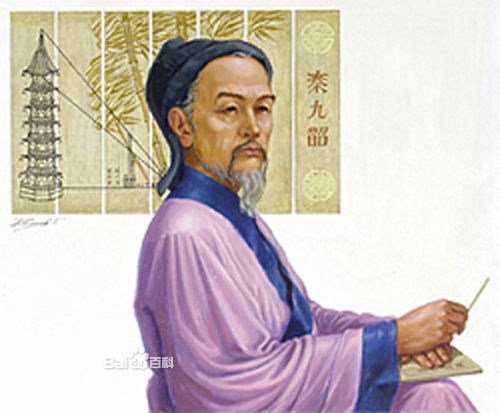
\includegraphics[width=4.0cm]{Chapters/Ch01/figure/qinjiushao.jpg}}
\end{minipage}
\hfill
\begin{minipage}{.6\linewidth}
\begin{itemize}
\item {数学九章}
\item {大衍求一术}
\item[] ~~比Gauss的同余理论早554年
\item  {任意次方程的数值解法}
\item[] ~~比英国人霍纳早提出572年
\item  {三斜求积术}
\item[] ~~海伦公式(公元50年左右)
\item {秦九韶公式}
\item {$\cd$}
\end{itemize}
\end{minipage}
\end{tabular}
\end{figure}
\end{frame}

%******
\begin{frame}\ft{原则3:避免两相近数相减} 
\begin{flushleft}
三、避免两个相近的数相减
\end{flushleft}
\pause 
数值计算中,两个相近的数相减会造成有效数字的严重丢失。
\pause 

\textcolor{acolor3}{处理办法}:
\begin{itemize}
\item
因式分解
\item
分子分母有理化
\item
三角函数恒等式
\item
Taylor展开式
\item
$\cdots$
\end{itemize}
 
\end{frame}
%
%
%
%******
\begin{frame}\ft{原则3:避免两相近数相减} 
\begin{li}
计算(取$4$位有效数字)
$$
\sqrt{x+1} -  \sqrt{x} ~~~~ (x = 1000)
$$
\end{li}
\pause
\begin{itemize}
\item
\textcolor{acolor5}{直接计算}
$$
\sqrt{1001} -  \sqrt{1000} \approx 31.64 - 31.62 = 0.02
$$
只有一个有效数字,损失了三位有效数字;\\[0.2cm]\pause
\item
\textcolor{acolor5}{分子有理化}
$$
\sqrt{x+1} -  \sqrt{x}  = \frac1{\sqrt{x+1} +  \sqrt{x}} \approx 0.01581
$$
没有损失有效数字。
\end{itemize}
\end{frame}

%
%******
\begin{frame}\ft{原则3:避免两相近数相减} 

\begin{li}
计算(取$4$位有效数字)
$$
A = 10^7(1-\cos 2^{\circ}) ~~~~ (\cos 2^{\circ} = 0.9994)
$$
\end{li}

\pause 
\begin{itemize}
\item
\textcolor{acolor5}{直接计算}
$$
A \approx 10^7(1-0.9994)  = 6 \times 10^3
$$
只有一个有效数字\\[0.2cm]\pause
\item
\textcolor{acolor5}{三角恒等式}
$\textcolor{acolor3}{\boxed{
  1 - \cos x = 2 \sin^2 \frac x2 
}}
$
$$
\begin{array}{ll}
A &= 10^7(1-\cos 2^{\circ})  = 2 \times (\sin 1^{\circ})^2 \times 10^7 \\[0.2cm]
&\approx 2 \times 0.01745^2 \times 10^7  \approx 6.09 \times 10^3
\end{array}
$$
三位有效数字
\end{itemize}
\end{frame}
%
%
%******
\begin{frame}\ft{原则4:避免绝对值很小的数做分母}%\fst{}

\begin{flushleft}
四、绝对值太小的数不宜做除数
\end{flushleft}
数值计算中,用绝对值很小的数作除数,会使商的数量级增加,甚至在计算机中造成“溢出”停机,
而且当很小的除数稍有一点误差,会对计算结果影响很大。
\pause 
\begin{li}
$$
\begin{array}{cl}
\ds \frac{3.1416}{0.001} & = 3141.6 \\[0.4cm]
\ds \frac{3.1416}{0.001+0.0001} & = 2856 
\end{array}
$$
\end{li}

\end{frame}



%******
\begin{frame}\ft{原则5:防止大数吃小数} 

\begin{flushleft}
五、合理安排运算次序,防止“大数吃小数”
\end{flushleft}

\begin{li}
计算$a, ~b, ~c$的和,其中$a = 10^{12}, ~b = 10, ~c \approx -a$.
\end{li}
\pause 

\begin{itemize}
\item
$(a+b)+c$
\item[]
~~~~结果接近于0; \pause
\item
$(a+c)+b$
\item[]
~~~~结果接近于10。
\end{itemize}

 
\end{frame}

\section{算法}

\begin{frame}
  \begin{figure}  
  \centering
  \begin{tikzpicture}
    The graphic
    \node at (0,0)[fill=red!20,draw,starburst,drop shadow,text width=0.5cm]{
      两种算法的比较
    };
    \pause
    \node at (1.5,1.5) [right,fill=blue!20,draw,rectangle,rounded corners=3mm,text width=4cm]{
\begin{lstlisting}[mathescape=true]
int i,sum=0,n=100;
for (i=1;i<=n;i++)
  sum=sum+i;
printf("%d",sum);
\end{lstlisting}
};
    \node at (1.5,-1.5) [right,fill=blue!20,draw,rectangle,rounded corners=3mm,text width=4cm]{
\begin{lstlisting}[mathescape=true]
int i,sum=0,n=100;
sum=(n+1)*n/2;
printf("%d",sum);
      \end{lstlisting}
    };
  \end{tikzpicture}
  
\end{figure}


    
\end{frame}

\begin{frame}
  \begin{figure}  
  \centering
  \begin{tikzpicture}
    The graphic
    \node at (0,0)[fill=blue!20,draw,starburst,drop shadow,text width=7cm]{
      \blue{\large 算法}\\
      算法是解决特定问题求解步骤的描述,在计算机中表现为指令的有限序列,并且每条指令表示一个或多个操作.
    };

  \end{tikzpicture}
  
\end{figure}


 
  \pause 
  \begin{figure}
    
\includegraphics[width=1in]{Chapters/Ch01/Fig/Hualazimi}
    \caption{阿勒.花剌子密(约780~约850,波斯数学家)}
  \end{figure}
\end{frame}

\begin{frame}
  \begin{figure}
  
  \centering
  \begin{tikzpicture}[scale=1.2]
    The graphic
    \node at (0,0)[fill=blue!20,draw,starburst,drop shadow,text width=0.8cm]{
      算法特性
    };
    \pause 
    \node at (0,2) [right,fill=red!20,draw,rectangle callout,callout relative pointer={(-0.6,-0.5)},rounded corners=3mm,text width=3cm]{ \small
      \blue{1、输入}\\
      有零个或多个输入
    };
    \pause 
    \node at (2,0.8) [right,fill=red!20,draw,ellipse callout,callout relative pointer={(-1.4,-0.3)},text width=3.6cm]{\small
      \blue{2、输出}\\
      至少有一个或多个输出
    };
    \pause 
    \node at (2,-1.2) [right,fill=red!20,draw,rectangle callout,callout relative pointer={(-1,0.1)},rounded corners=3mm,text width=5cm]{\small
      \blue{3、有穷性}\\
      在执行有限步后,会自动结束而不出现无限循环,并且每一步在可接受的时间内完成
    };
    \pause 
    \node at (1,-3.5) [right,fill=red!20,draw,ellipse callout,callout relative pointer={(-2.2,1.5)},text width=4cm]{\small
      \blue{4、确定性}\\
      每一步都有确定的含义,不出现二义性
    };
    \pause 
    \node at (-2,-3) [right,fill=red!20,draw,rectangle callout,callout relative pointer={(0.3,0.7)},rounded corners=3mm,text width=2.5cm]{\small
      \blue{5、可行性}\\
      每一步都必须可行,能通过执行有限次数完成
    };
  \end{tikzpicture}  
\end{figure}
    
  
\end{frame}


\begin{frame}
  \documentclass{article}
\usepackage{CJK} 
\usepackage{graphics}
\usepackage{pgf}
\usepackage{tikz}
\usetikzlibrary{calc,shadows}
\usetikzlibrary{decorations.markings,scopes}
\usetikzlibrary{arrows,snakes,backgrounds,shapes}
\usetikzlibrary{decorations.pathmorphing}
\usepackage{listings}
\renewcommand{\ttdefault}{pcr}
\lstset{
  keywordstyle=\color{blue!70},
  frame=single,
  basicstyle=\ttfamily\bfseries\small,
  commentstyle=\small\color{red},
  rulesepcolor=\color{red!20!green!20!blue!20},
  tabsize=4,
  numbersep=5pt,
  %% backgroundcolor=\color{black!10},
  showspaces=false,
  showtabs=false,
  extendedchars=false,
  escapeinside=``,
  frame=no
}

\newcommand{\blue}{\textcolor{blue}}
\newcommand{\red}{\textcolor{red}}
\newcommand{\purple}{\textcolor{purple}}


\pgfrealjobname{survey}
\begin{document}
\begin{CJK}{UTF8}{gkai} 
  \beginpgfgraphicnamed{AlgDesign}
  \begin{tikzpicture}
    The graphic
    \node at (0,0)[fill=blue!20,draw,starburst,drop shadow,text width=0.8cm]{
      算法设计要求
    };
    %% \node at (0,2) [right,fill=red!20,draw,rectangle callout,callout relative pointer={(-0.6,-0.5)},rounded corners=3mm,text width=3cm]{ 
    \node at (1.5,0) [right,fill=red!20,draw,rectangle split, rectangle split parts=4,rounded corners=3mm,text width=7cm]{
      \blue{正确性}\\
      算法至少应该具有输入、输出和加工处理无歧义性,能正确反映问题的需求、能得到问题的正确答案。
      \begin{itemize}
      \item 无语法错误
      \item 对合法输入能产生满足要求的输出
      \item 对非法输入能给出满足规格的说明
      \item 对精心选择的甚至是刁难的测试数据都有满足要求的输出
      \end{itemize}
      \nodepart{second}
      \blue{可读性}\\
      便于阅读、理解和交流
      \nodepart{third}
      \blue{健壮性}\\
      当输入不合法时,也能做出相应处理,而不是产生异常或莫名其妙的结果
      \nodepart{fourth}
      \blue{时间效率高和存储量低}
    };   
  \end{tikzpicture}
  \endpgfgraphicnamed  
\end{CJK}

\end{document}


    
  
\end{frame}

\begin{frame}
  \begin{figure}
  
  \centering
    \begin{tikzpicture}
    The graphic
    \node at (0,0)[fill=blue!20,draw,starburst,drop shadow,text width=0.8cm]{
      算法效率度量方法
    };
    \pause 
    %% \node at (0,2) [right,fill=red!20,draw,rectangle callout,callout relative pointer={(-0.6,-0.5)},rounded corners=3mm,text width=3cm]{ 
    \node at (2,1) [right,fill=red!20,draw,ellipse callout,callout relative pointer={(-0.8,-0.1)},text width=3cm]{
      \blue{事后统计方法}
    };
    \pause 
    \node at (2,-1) [right,fill=red!20,draw,ellipse callout,callout relative pointer={(-0.8,0.1)},text width=3cm]{
      \blue{事前分析估算方法}
    };

  \end{tikzpicture}
\end{figure}
    
  
\end{frame}

\begin{frame}
  \begin{figure}
  
  \centering
  \begin{tikzpicture}[node distance=4.5cm]
    \node [fill=blue!20,draw,starburst,drop shadow,text width=7.5cm] (1) {
      \blue{\large 事后统计方法}\\
      通过设计好的测试程序和数据,利用计算机计时器对不同算法编制的程序的运行时间进行比较,从而确定效率的高低。
    };
    \pause 
    \node[below of=1,rectangle split,rectangle split parts=4,rounded corners=3mm,draw,text width=10cm,fill=red!20] {
      \blue{缺点}
      \nodepart{second}
      须依据算法事先编制好程序
      \nodepart{third}
      时间的比较依赖于软硬件等环境因素\\
      \begin{itemize}
      \item 不同性能的机器上算法的表现不尽相同;
      \item 不同操作系统、编译器等也会影响算法的运行结果;\\
      \item CPU使用率和内存占用情况也会造成微小差异。
      \end{itemize}
      \nodepart{fourth}
      测试数据设计困难,且程序运行时间还与测试数据的规模有很大关系,
      效率高的算法在小的测试数据面前往往得不到体现。
    };

  \end{tikzpicture}  
\end{figure}
    
  
\end{frame}

\begin{frame}
  \begin{figure}
  
  \centering
    \begin{tikzpicture}[node distance=6cm]
  \node [fill=blue!20,draw,starburst,drop shadow,text width=5cm] (1) {
  \blue{\large 事前分析估算方法}\\
  在编制程序前,依据统计方法对算法进行估算。
  };
  \pause
  
  \node[below left of=1,rectangle split,rectangle split parts=5,rounded corners=3mm,draw,text width=7cm,fill=red!20] (2){
    \blue{程序运行时间取决于}
      \nodepart{two}
      (1)~算法采用的策略、方法 (\red{算法好坏的根本})
      \nodepart{three}
      (2)~编译产生的代码质量 (\red{软件支持})
      \nodepart{four}
      (3)~问题的输入规模 
      \nodepart{five}
      (4)~机器执行指令的速度 (\red{硬件性能})
    };
  \pause
    \node[right of=2,rectangle split,ellipse,draw,text width=2.5cm,fill=red!20] {
      程序的运行时间,依赖于算法的好坏和问题的输入规模。
    };

  \end{tikzpicture}

\end{figure}
    
  
\end{frame}

\begin{frame}
  \begin{figure}
  \centering
  \begin{tikzpicture}[node distance=2.5cm]

    \node[rectangle split,rectangle split parts=3,rounded corners=3mm,draw,text width=7cm,fill=red!20](1){
\begin{lstlisting}[language=C,mathescape]
for(i=1;i<=n;i++)
  sum+=i;          //`执行$n$次`
\end{lstlisting}
\nodepart{two}
\begin{lstlisting}[language=C]
sum=(n+1)*n/2;     //`执行$1$次`
\end{lstlisting}
\nodepart{three}
\begin{lstlisting}[language=C]
for(i=1;i<=n;i++)
  for(j=1;j<=n;j++){
    x++;           //`执行$n\times n$次`
    sum+=x;
  }
\end{lstlisting}
    };
    
  \end{tikzpicture}
\end{figure}


    
\end{frame}

\begin{frame}
  \documentclass{article}
\usepackage{CJK} 
\usepackage{graphics}
\usepackage{pgf}
\usepackage{pgfplots}
\usepackage{tikz}
\usetikzlibrary{calc,shadows}
\usetikzlibrary{decorations.markings,scopes}
\usetikzlibrary{arrows,snakes,backgrounds,shapes}
\usetikzlibrary{decorations.pathmorphing}
\usepackage{listings}
\renewcommand{\ttdefault}{pcr}
\lstset{
  keywordstyle=\color{blue!70},
  frame=single,
  basicstyle=\ttfamily\bfseries\small,
  commentstyle=\small\color{red},
  rulesepcolor=\color{red!20!green!20!blue!20},
  tabsize=4,
  numbersep=5pt,
  %% backgroundcolor=\color{black!10},
  showspaces=false,
  showtabs=false,
  extendedchars=false,
  escapeinside=``,
  frame=no
}

\newcommand{\blue}{\textcolor{blue}}
\newcommand{\red}{\textcolor{red}}
\newcommand{\purple}{\textcolor{purple}}


\pgfrealjobname{survey}
\begin{document}
\begin{CJK}{UTF8}{gkai} 
  \beginpgfgraphicnamed{AlgEffBefore2}
  \begin{tikzpicture}[node distance=2.5cm]

    \begin{axis}[
        xmin=0, xmax=12,
        ymin=0, ymax=120,
        extra x ticks={2,4,6,8,10},
        extra y ticks={20,40,60,80,100},
        extra tick style={grid=major},
        ylabel=算法实际操作数量,
        xlabel=问题输入规模$n$,
        legend style={at={(1,0.5)},anchor=east}
      ]
      \addplot[domain=1:10,purple]{1};
      \addplot[domain=1:10,blue]{x};
      \addplot[domain=1:10,red]{x*x};
      \legend{$1$,$n$,$n^2$}
    \end{axis}
    
  \end{tikzpicture}
  \endpgfgraphicnamed  
\end{CJK}

\end{document}


    
  
\end{frame}

\begin{frame}
  \documentclass{article}
\usepackage{amsmath,amssymb,amsfonts}
\usepackage{CJK} 
\usepackage{graphics}
\usepackage{pgf}
\usepackage{tikz}
\usetikzlibrary{calc,shadows}
\usetikzlibrary{decorations.markings,scopes}
\usetikzlibrary{arrows,snakes,backgrounds,shapes}
\usetikzlibrary{decorations.pathmorphing}
\usepackage{listings}
\renewcommand{\ttdefault}{pcr}
\lstset{
  keywordstyle=\color{blue!70},
  frame=single,
  basicstyle=\ttfamily\bfseries\small,
  commentstyle=\small\color{red},
  rulesepcolor=\color{red!20!green!20!blue!20},
  tabsize=4,
  numbersep=5pt,
  %% backgroundcolor=\color{black!10},
  showspaces=false,
  showtabs=false,
  extendedchars=false,
  escapeinside=``,
  frame=no
}

\newcommand{\blue}{\textcolor{blue}}
\newcommand{\red}{\textcolor{red}}
\newcommand{\purple}{\textcolor{purple}}


\pgfrealjobname{survey}
\begin{document}
\begin{CJK}{UTF8}{gkai} 
  \beginpgfgraphicnamed{FuncAymInc}
  \begin{tikzpicture}[node distance=4.3cm]
  \node [fill=blue!20,draw,starburst,drop shadow,text width=6cm] (1) {
  \blue{\large 函数的渐近增长}\\
  给定两个函数$f(n)$和$g(n)$,若$\exists N \in \mathbb N$, s.t. $\forall n>N$, $f(n)$总是比$g(n)$大,
  我们就说$f(n)$的增长渐近快于$g(n)$.
  };
  \end{tikzpicture}
  \endpgfgraphicnamed  
\end{CJK}

\end{document}


    
  \pause 

  \begin{table}
    \begin{tabular}{|l|r|r|r|r|}\hline
      次数$n$&算法$A$&算法$A^\prime$&算法$B$&算法$B^\prime$\\
      & $(2n+3)$&$(2n)$&$(3n+1)$&$(3n)$\\\hline
      1  &  5&  2&  4&  3\\\hline
      2  &  7&  4&  7&  6\\\hline
      3  &  9&  6& 10&  9\\\hline
      10 & 23& 20& 31& 30\\\hline
      100&203&200&301&300\\\hline      
    \end{tabular}
  \end{table}
\end{frame}


\begin{frame}
  \begin{table}
    \begin{tabular}{|l|r|r|r|r|}\hline
      次数$n$&算法$C$&算法$C^\prime$&算法$D$&算法$D^\prime$\\
      & $(4n+8)$&$(n)$&$(2n^2+1)$&$(n^2)$\\\hline
      1   &   12&    1&        3&        2\\\hline
      2   &   16&    2&        9&        4\\\hline
      3   &   20&    3&       19&        9\\\hline
      10  &   48&   10&      201&      100\\\hline
      100 &  408&  100&   20 001&   10 000\\\hline
      1000&4 008&1 000&2 000 001&1 000 000\\\hline      
    \end{tabular}
  \end{table}
  \pause
  \documentclass{article}
\usepackage{CJK} 
\usepackage{graphics}
\usepackage{pgf}
\usepackage{tikz}
\usetikzlibrary{calc,shadows}
\usetikzlibrary{decorations.markings,scopes}
\usetikzlibrary{arrows,snakes,backgrounds,shapes}
\usetikzlibrary{decorations.pathmorphing}
\usepackage{listings}
\renewcommand{\ttdefault}{pcr}
\lstset{
  keywordstyle=\color{blue!70},
  frame=single,
  basicstyle=\ttfamily\bfseries\small,
  commentstyle=\small\color{red},
  rulesepcolor=\color{red!20!green!20!blue!20},
  tabsize=4,
  numbersep=5pt,
  %% backgroundcolor=\color{black!10},
  showspaces=false,
  showtabs=false,
  extendedchars=false,
  escapeinside=``,
  frame=no
}

\newcommand{\blue}{\textcolor{blue}}
\newcommand{\red}{\textcolor{red}}
\newcommand{\purple}{\textcolor{purple}}


\pgfrealjobname{survey}
\begin{document}
\begin{CJK}{UTF8}{gkai} 
  \beginpgfgraphicnamed{FuncAymInc1}
  \begin{tikzpicture}
    \node at (1.5,1) [right,fill=red!20,draw,ellipse callout,callout relative pointer={(-0.8,0.2)},text width=5cm,text=blue]{
      函数的渐近增长可忽略加法常数,并且最高次项的系数也不重要。
    };
  \end{tikzpicture}
  \endpgfgraphicnamed  
\end{CJK}

\end{document}


    
  

\end{frame}


\begin{frame}
  \begin{table}
    \begin{tabular}{|l|r|r|r|r|}\hline
      次数$n$&算法$E$&算法$E^\prime$&算法$F$&算法$F^\prime$\\
      &$(2n^2+3n+1)$&$(n^2)$&$(2n^3+3n+1)$&$(n^3)$\\
      \hline
      1   &     6&     1&        6&        1\\\hline
      2   &    15&     4&       23&        8\\\hline
      3   &    28&     9&       64&       27\\\hline
      10  &   231&   100&    2 031&    1 000\\\hline
      100 &20 301&10 000&2 000 301&1 000 000\\\hline
    \end{tabular}
  \end{table}

  \pause
  \documentclass{article}
\usepackage{CJK} 
\usepackage{graphics}
\usepackage{pgf}
\usepackage{tikz}
\usetikzlibrary{calc,shadows}
\usetikzlibrary{decorations.markings,scopes}
\usetikzlibrary{arrows,snakes,backgrounds,shapes}
\usetikzlibrary{decorations.pathmorphing}
\usepackage{listings}
\renewcommand{\ttdefault}{pcr}
\lstset{
  keywordstyle=\color{blue!70},
  frame=single,
  basicstyle=\ttfamily\bfseries\small,
  commentstyle=\small\color{red},
  rulesepcolor=\color{red!20!green!20!blue!20},
  tabsize=4,
  numbersep=5pt,
  %% backgroundcolor=\color{black!10},
  showspaces=false,
  showtabs=false,
  extendedchars=false,
  escapeinside=``,
  frame=no
}

\newcommand{\blue}{\textcolor{blue}}
\newcommand{\red}{\textcolor{red}}
\newcommand{\purple}{\textcolor{purple}}


\pgfrealjobname{survey}
\begin{document}
\begin{CJK}{UTF8}{gkai} 
  \beginpgfgraphicnamed{FuncAymInc2}
  \begin{tikzpicture}
    \node at (1.5,1) [right,fill=red!20,draw,ellipse callout,callout relative pointer={(-0.8,0.2)},text width=5cm,text=blue]{
      最高次项的指数越大,随着$n$的增长,函数结果也会变得增长特别快。
    };
  \end{tikzpicture}
  \endpgfgraphicnamed  
\end{CJK}

\end{document}


    
  

\end{frame}


\begin{frame}
  \begin{table}
    \begin{tabular}{|l|r|r|r|r|}\hline
      次数$n$&算法$G$&算法$H$&算法$I$\\
            &$(2n^2)$&$(3n+1)$&$(2n^2+3n+1)$\\
      \hline
      1        &                2&        4&                 6\\\hline
      2        &                8&        7&                15\\\hline
      5        &               50&       16&                66\\\hline
      10       &              200&       31&               231\\\hline
      100      &           20 000&      301&            20 301\\\hline
      1,000    &        2 000 000&    3 001&         2 003 001\\\hline
      10,000   &      200 000 000&   30 001&       200 030 001\\\hline
      100,000  &   20 000 000 000&  300 001&    20 000 300 001\\\hline
      1,000,000&2 000 000 000 000&3 000 001& 2 000 003 000 001\\\hline
    \end{tabular}
  \end{table}
  \pause
  \begin{zhu}
    当$n$越来越大时,$3n+1$的结果与$2n^2$相比,几乎可以忽略不计。也就是说,随着$n$的不断增大,
    算法$G$其实很接近于算法$I$.
  \end{zhu}

\end{frame}


\begin{frame}


  \documentclass{article}
\usepackage{CJK} 
\usepackage{graphics}
\usepackage{pgf}
\usepackage{tikz}
\usetikzlibrary{calc,shadows}
\usetikzlibrary{decorations.markings,scopes}
\usetikzlibrary{arrows,snakes,backgrounds,shapes}
\usetikzlibrary{decorations.pathmorphing}
\usepackage{listings}
\renewcommand{\ttdefault}{pcr}
\lstset{
  keywordstyle=\color{blue!70},
  frame=single,
  basicstyle=\ttfamily\bfseries\small,
  commentstyle=\small\color{red},
  rulesepcolor=\color{red!20!green!20!blue!20},
  tabsize=4,
  numbersep=5pt,
  %% backgroundcolor=\color{black!10},
  showspaces=false,
  showtabs=false,
  extendedchars=false,
  escapeinside=``,
  frame=no
}

\newcommand{\blue}{\textcolor{blue}}
\newcommand{\red}{\textcolor{red}}
\newcommand{\purple}{\textcolor{purple}}


\pgfrealjobname{survey}
\begin{document}
\begin{CJK}{UTF8}{gkai} 
  \beginpgfgraphicnamed{FuncAymInc3}
  \begin{tikzpicture}
    \node [fill=blue!20,draw,starburst,drop shadow,text width=6cm] (1) {
      判断一个算法的效率时,函数中的常数与其他次要项可以忽略,而更应该关注主项(最高阶项)的阶数。
    };
  \end{tikzpicture}
  \endpgfgraphicnamed  
\end{CJK}

\end{document}


    
  

\end{frame}


\begin{frame}
  \begin{figure}
  \centering
  \begin{tikzpicture}[node distance=4cm]
    \node [fill=blue!20,draw,starburst,drop shadow,text width=3.5cm,text=blue] (1) {
      {\large 算法时间复杂度}
    };
    \node [below of=1,fill=red!20,draw,rectangle,rounded corners=4mm,text width=7.8cm] (2) {
      在进行算法分析时,语句总的执行次数$T(n)$是关于问题规模$n$的函数,
      进而分析$T(n)$随$n$的变化情况并确定$T(n)$的数量级。算法的时间复杂度,也就是算法的时间量度,
      记作
      $$
      T(n)=O(f(n)).
      $$
      它表示随着$n$的增大,算法执行时间的增长率和$f(n)$的增长率相同,称为算法的渐近时间复杂度,
      简称为时间复杂度,其中$f(n)$是关于$n$的某个函数。
    };

    \pause 
    \node at (1.6,-3.5)[right,fill=green!20,draw,ellipse callout,callout relative pointer={(-0.8,-0.2)},text width=2cm,text=blue]{
      大O记法
    };
  \end{tikzpicture}
  
\end{figure}
    
\end{frame}

\begin{frame}
  \begin{figure}
  \centering
  \begin{tikzpicture}[node distance=3.2cm]
    \node [fill=blue!20,draw,starburst,drop shadow,text width=6cm,text=blue] (1) {
      如何分析一个算法的时间复杂度?即如何推导大O阶?
    };

    \pause 
    \node [below of=1,fill=red!20,draw,rectangle split,rectangle split parts=4,rounded corners=4mm,text width=8.5cm,text=blue]{
      1.~用常数1取代运行次数中的所有加法常数;
      \nodepart{two}
      2.~在修改后的运行次数函数中,只保留最高阶项;
      \nodepart{three}
      3.~如果最高阶项存在且不是1,则去除最高阶项的系数。
      \nodepart{four}
      得到的结果就是大O阶。
    };
  \end{tikzpicture}
  
\end{figure}
    
\end{frame}


\begin{frame}
  \begin{figure}
  \centering
  \begin{tikzpicture}[node distance=2cm]
    \node [fill=blue!20,draw,starburst,drop shadow,text width=2cm,text=blue] (1) {
      常数阶$O(1)$
    };

    \node [below of=1,fill=red!20,draw,rectangle,rounded corners=4mm,text width=8cm,text=blue]{
      \begin{lstlisting}[language=C]
int sum=0,n=100;  //`执行1次`
sum=(n+1)*n/2;    //`执行1次`
printf("%d",sum); //`执行1次`
      \end{lstlisting}
    };
  \end{tikzpicture}
\end{figure}

    
\end{frame}

\begin{frame}
  \begin{figure}
  \centering
  \begin{tikzpicture}[node distance=3cm]
    \node [fill=blue!20,draw,starburst,drop shadow,text width=2cm,text=blue] (1) {
      常数阶$O(1)$
    };

    \node [below of=1,fill=red!20,draw,rectangle,rounded corners=4mm,text width=8cm,text=blue]{
      \begin{lstlisting}[language=C]
int sum=0,n=100;  //`执行1次`
sum=(n+1)*n/2;    //`执行第1次`
sum=(n+1)*n/2;    //`执行第2次`
sum=(n+1)*n/2;    //`执行第3次`
sum=(n+1)*n/2;    //`执行第4次`
sum=(n+1)*n/2;    //`执行第5次`
printf("%d",sum); //`执行1次`
      \end{lstlisting}
    };
  \end{tikzpicture}
\end{figure}


    
\end{frame}


\begin{frame}
  \documentclass{article}
\usepackage{CJK} 
\usepackage{graphics}
\usepackage{pgf}
\usepackage{tikz}
\usetikzlibrary{calc,shadows}
\usetikzlibrary{decorations.markings,scopes}
\usetikzlibrary{arrows,snakes,backgrounds,shapes}
\usetikzlibrary{decorations.pathmorphing}
\usepackage{listings}

\lstset{
  keywordstyle=\color{blue!70},
  frame=single,
  basicstyle=\ttfamily\small,
  commentstyle=\small\color{red},
  rulesepcolor=\color{red!20!green!20!blue!20},
  tabsize=4,
  numbersep=5pt,
  %% backgroundcolor=\color{black!10},
  showspaces=false,
  showtabs=false,
  extendedchars=false,
  escapeinside=``,
  frame=no
}

\newcommand{\blue}{\textcolor{blue}}
\newcommand{\red}{\textcolor{red}}
\newcommand{\purple}{\textcolor{purple}}


\pgfrealjobname{survey}
\begin{document}
\begin{CJK}{UTF8}{gkai} 
  \beginpgfgraphicnamed{LinOrder}
  \begin{tikzpicture}[node distance=3cm]
    \node [fill=blue!20,draw,starburst,drop shadow,text width=2cm,text=blue] (1) {
      线性阶$O(n)$
    };

    \node [below of=1,fill=red!20,draw,rectangle,rounded corners=4mm,text width=6cm,text=blue]{
      \begin{lstlisting}[language=C]
int i;
for (i=0;i<n;i++}
    //`时间复杂度为$O(1)$的语句块`
      \end{lstlisting}
    };
  \end{tikzpicture}
  
  \endpgfgraphicnamed  
\end{CJK}

\end{document}


    
  
\end{frame}

\begin{frame}
  \begin{figure}
  \centering
  \begin{tikzpicture}[node distance=2.8cm]
    \node [fill=blue!20,draw,starburst,drop shadow,text width=3cm,text=blue]
    (1) {
      对数阶$O(\log n)$
    };

    \node [below of=1,fill=red!20,draw,rectangle,rounded corners=4mm,text width=6cm,text=blue]
    (2) {
      \begin{lstlisting}[language=C,frame=no]
int count=1;
while (count<n){
  count*=2;
  //`时间复杂度为$O(1)$的语句块`
}
      \end{lstlisting}
    };
\pause 
    \node [below of=2,fill=green!40,draw,rectangle callout,callout relative pointer={(-0.5,1)},rounded corners=4mm,text width=8cm,text=blue]
    (3) {
      $$
      2^x=n ~\Longrightarrow ~
      x=\log_2 n 
      = \frac{\log n}{\log 2}.
      $$
    };
    
  \end{tikzpicture}
\end{figure}  


    
\end{frame}

\begin{frame}
  \begin{figure}
  \centering
  \begin{tikzpicture}[node distance=4.6cm]
    
    
    \node [fill=red!20,draw,rectangle split,rectangle split parts=3,rounded corners=4mm,text width=6cm,text=blue]
    (2){
      \begin{lstlisting}[language=C,frame=no]
int i,j;
for (i=0;i<n;i++)
  for (j=0;j<n;j++)
    //`时间复杂度为$O(1)$的语句块`
      \end{lstlisting}
      \nodepart{two}
      \begin{lstlisting}[language=C,frame=no]
int i,j;
for (i=0;i<m;i++)
  for (j=0;j<n;j++)
    //`时间复杂度为$O(1)$的语句块`
      \end{lstlisting}
      \nodepart{three}
      \begin{lstlisting}[language=C,frame=no]
int i,j;
for (i=0;i<n;i++)
  for (j=i;j<n;j++)
    //`时间复杂度为$O(1)$的语句块`
      \end{lstlisting}
    };

    \node at(5,4) [fill=blue!20,draw,starburst,drop shadow,text width=3cm,text=blue]
    (1) {
      平方阶$O(n^2)$
    };
    \pause 
    \node at (4.8,2.2)[fill=green!40,draw,ellipse callout,callout relative pointer={(-1,0.5)},text width=1cm,text=blue]
    (3) {
      $O(n^2)$
    };

    \pause 
    \node at (4.8,0)[fill=green!40,draw,ellipse callout,callout relative pointer={(-1,-0.5)},text width=2cm,text=blue]
    (4) {
      $O(m\times n)$
    };

    \pause 
    \node at (4.6,-2)[fill=green!40,draw,rectangle callout,callout relative pointer={(-0.7,-0.2)},rounded corners=3mm,text width=7.5cm,text=blue]
    (5) {
      因$f(n)=n+\cdots+2+1=\frac{n(n+1)}{2}=\frac{n^2}2+\frac n2$,
      故时间复杂度为$O(n^2)$.
    };


  \end{tikzpicture}
\end{figure}

    
\end{frame}

\begin{frame}
  \begin{figure}
  \centering
  \begin{tikzpicture}[node distance=4cm]
    \node [fill=red!20,draw,rectangle split,rectangle split parts=2,rounded corners=4mm,text width=6cm,text=blue]
    (1){
      \begin{lstlisting}[language=C,frame=no]
int i,j;        
for (i=0;i<n;i++)
  function(i);
      \end{lstlisting}
      \nodepart{two}
      \begin{lstlisting}[language=C,frame=no]
void function(int i){
  print("%d",i);
}
      \end{lstlisting}
    }; 
    \node [below right of=1,fill=orange!40,draw,ellipse callout,callout relative pointer={(-2,0.6)},text width=3.5cm,text=blue]
    (2) {
      请分析时间复杂度.
    };
    \pause 
    \node [below of=1,fill=green!40,draw,ellipse callout,callout relative pointer={(-0.7,1.8)},text width=1cm,text=blue]
    (2) {
      $O(n)$
    };

  \end{tikzpicture}
\end{figure}

\end{frame}

\begin{frame}
  \begin{figure}
  \centering
  \begin{tikzpicture}[node distance=4cm]
    \node [fill=red!20,draw,rectangle split,rectangle split parts=2,rounded corners=4mm,text width=6cm,text=blue]
    (1){
      \begin{lstlisting}[language=C,frame=no]
int i,j;        
for (i=0;i<n;i++)
  function(i);
      \end{lstlisting}
      \nodepart{two}
      \begin{lstlisting}[language=C,frame=no]
void function(int i){
  int j;
  for (j=i;j<n;j++)
    //`时间复杂度为$O(1)$的语句块`
}
      \end{lstlisting}
    }; 
    \node [below right of=1,fill=orange!40,draw,ellipse callout,callout relative pointer={(-2,0.6)},text width=3.5cm,text=blue]
    (2) {
      请分析时间复杂度.
    };
    \pause 
    \node [below of=1,fill=green!40,draw,ellipse callout,callout relative pointer={(-0.7,1.8)},text width=1cm,text=blue]
    (2) {
      $
      O(n^2)
      $
    };

  \end{tikzpicture}
\end{figure}

\end{frame}

\begin{frame}
  \begin{figure}
  \centering
  \begin{tikzpicture}[node distance=4cm]
    \node [fill=red!20,draw,rectangle,rounded corners=4mm,text width=10cm,text=blue]
    (1){
      \begin{lstlisting}[language=C,frame=no]
n++;                 //`执行次数为$1$`
function(n);         //`执行次数为$n$`
int i,j;  
for (i=0;i<n;i++)    //`执行次数为$n^2$`
  function(i);
for (i=0;i<n;i++)   //`执行次数为$n(n+1)/2$`
  for (j=i;j<n;j++)
    //`时间复杂度为$O(1)$的语句块`
      \end{lstlisting}
    }; 
    \node [below right of=1,fill=orange!40,draw,ellipse callout,callout relative pointer={(-2,0.6)},text width=3.5cm,text=blue]
    (2) {
      请分析时间复杂度.
    };
    \pause 
    \node [below of=1,fill=green!40,draw,rectangle callout,callout relative pointer={(-0.7,1.8)},rounded corners=3mm,text width=8.5cm,text=blue]
    (2) {
      执行次数$f(n)=1+n+n^2+\frac{n(n+1)}2=\frac32n^2+\frac32n+1$,
      故时间复杂度为$O(n^2)$.
    };

  \end{tikzpicture}
\end{figure}

\end{frame}


\begin{frame}
  \begin{table}
    \caption{常见时间复杂度}
    \begin{tabular}{l|l|l}\hline
      执行次数函数&阶&非正式术语\\\hline
      $12$&$O(1)$&常数阶\\[0.05in]
      $2n+3$&$O(n)$&线性阶\\[0.05in]
      $3n^2+2n+1$&$O(n^2)$&平方阶\\[0.05in]
      $5\log_2n+20$&$O(\log n)$&对数阶\\[0.05in]
      $2n+3n\log_2n+19$&$O(n\log n)$&$n\log n$阶\\[0.05in]
      $6n^3+2n^2+3n+4$&$O(n^3)$&立方阶\\[0.05in]
      $2^n$&$O(2^n)$&指数阶\\\hline
    \end{tabular}
  \end{table}
  \pause 
  \begin{figure}
    \centering
    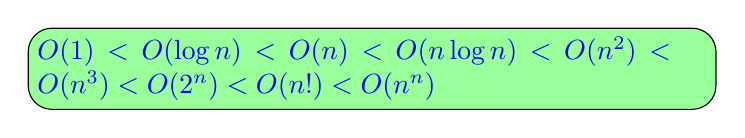
\begin{tikzpicture}
      \node [fill=green!40,draw,rectangle,rounded corners=3mm,text width=8.5cm,text=blue]
      (2) {
        $O(1)<O(\log n)<O(n)<O(n\log n)<O(n^2)<O(n^3)<O(2^n)<O(n!)<O(n^n)$
      };
    \end{tikzpicture}        
  \end{figure}
\end{frame}


\begin{frame}
  \begin{figure}
  \centering
  \begin{tikzpicture}[node distance=4cm]
    \node [fill=blue!20,draw,starburst,drop shadow,text width=2cm,text=blue] (1) {
      {\large 最坏情况}
    };
    \node [below left of=1,fill=red!20,draw,rectangle,rounded corners=4mm,text width=5.5cm] (2) {
      在$n$维随机数组中查找某个数字,
      \begin{itemize}
      \item 最好情况是出现在第一个位置,时间复杂度为$O(1)$;
      \item 最坏情况是出现在最后一个位置,时间复杂度为$O(n)$.
      \end{itemize}
    };

    \pause 
    \node at (3,-5)[text width=4.5cm,decorate,decoration=saw,fill=blue!20,draw,circle]{
      最坏情况运行时间是一种保证,亦即运行时间将不会再坏了。在应用中,这是一种最重要的需求,通常,除非特别指定,我们提到的运行时间都是最坏情况的运行时间。
    };
  \end{tikzpicture}
  
\end{figure}

\end{frame}

\begin{frame}
  \begin{figure}
  \centering
  \begin{tikzpicture}[node distance=4cm]
    \node [fill=blue!20,draw,starburst,drop shadow,text width=2cm,text=blue] (1) {
      {\large 平均情况}
    };
    \node [below left of=1,fill=red!20,draw,rectangle,rounded corners=4mm,text width=5.5cm] (2) {
      在$n$维随机数组中查找某个数字,
      \begin{itemize}
      \item 从概率角度讲,该数字在每个位置的可能性相同,故平均查找时间为$n/2$。
      \end{itemize}
    };

    \pause 
    \node at (3,-5)[text width=4.5cm,decorate,decoration=saw,fill=blue!20,draw,circle]{
      平均运行时间是所有情况中最有意义的,因为它是期望的运行时间。
    };
  \end{tikzpicture}
  
\end{figure}

\end{frame}

\begin{frame}
  \begin{figure}
  \centering
  \begin{tikzpicture}[node distance=3cm]
    \node [fill=blue!20,draw,starburst,drop shadow,text width=1cm,text=blue] (1) {
      {\large 小结}
    };
    \node [below of=1,fill=red!20,draw,rectangle,rounded corners=4mm,text width=9cm] (2) {
      对算法的分析,
      \begin{itemize}
      \item 一种方法是计算所有情况的平均值,这种时间复杂度的计算方法称为\blue{平均时间复杂度};
      \item 另一种是计算最坏情况下的时间复杂度,这种方法称为\blue{最坏时间复杂度}。
      \end{itemize}
      在没有特别说明的情况下,都指最坏时间复杂度。
    };

  \end{tikzpicture}
  
\end{figure}


\end{frame}

\begin{frame}
  \begin{figure}
  \centering
  \begin{tikzpicture}[node distance=4cm]
    \node [fill=blue!20,draw,starburst,drop shadow,text width=3.5cm,text=blue] (1) {
      {\large 算法空间复杂度}
    };
    \node [below of=1,fill=red!20,draw,rectangle,rounded corners=4mm,text width=7.8cm] (2) {
      通过计算算法所需的存储空间实现,其计算公式记作
      $$
      S(n)=O(f(n)).
      $$
      其中$n$为问题的规模,$f(n)$是语句关于$n$所占存储空间的函数。
    };
  \end{tikzpicture}
  
\end{figure}

\end{frame}

\begin{frame}
  \begin{figure}
  \centering
  \begin{tikzpicture}[node distance=0.8cm]
    \node at(0,0) [fill=blue!20,draw,starburst,drop shadow,text width=2cm,text=blue,text centered] (1) {
      {\large 总结回顾}
    };
    \pause 
    \node at(0,-1.5) [fill=red!20,draw,rectangle,rounded corners=2mm,text width=10cm,text centered] (2) {
      数据
    };
    \pause 
    \node [below of=2,fill=red!20,draw,rectangle,rounded corners=2mm,text width=10cm,text centered] (3) {
      数据对象
    };
    \pause 
    \node [below of=3,fill=red!20,draw,rectangle split,rectangle split parts=4,rectangle split horizontal,
      rounded corners=2mm,text width=2.3cm,text centered] (4) {
      数据元素 \nodepart{two}
      数据元素 \nodepart{three}
      数据元素 \nodepart{four}
      数据元素 
    };
    \pause 
    \node [below of=4,fill=red!20,draw,rectangle split,rectangle split parts=8,rectangle split horizontal,
      rounded corners=2mm,text width=1cm,text centered] (4) {
      \scriptsize{数据项1} \nodepart{two}
      \scriptsize{数据项2} \nodepart{three}
      \scriptsize{数据项1} \nodepart{four}
      \scriptsize{数据项2} \nodepart{five}
      \scriptsize{数据项1} \nodepart{six}
      \scriptsize{数据项2} \nodepart{seven}
      \scriptsize{数据项1} \nodepart{eight}
      \scriptsize{数据项2} 
    }; \pause 
    \node at (0,-6) [fill=green!40,draw,ellipse,rounded corners=2mm,text width=6cm,text centered]{
      数据结构是相互之间存在一种或多种特定关系的数据元素的集合。
    };

  \end{tikzpicture}
  
\end{figure}




\end{frame}

\begin{frame}
  \begin{figure}
  \centering
  \begin{tikzpicture}[node distance=4cm]
    \node at(0,0) [fill=blue!20,draw,starburst,drop shadow,text width=2cm,text=blue,text centered] (1) {
      {\large 总结回顾}
    };
    \pause     
    \node[below left of=1,fill=green!20,draw,rectangle split,rectangle split parts=5,rounded corners=2mm,text width=4cm,text centered,text=blue] (2) {
      \red{逻辑结构} \nodepart{two}
      集合结构 \nodepart{three}
      线性结构 \nodepart{four}
      树形结构 \nodepart{five}
      图形结构 
    };
    \pause 
    \node[below right of=1,fill=green!20,draw,rectangle split,rectangle split parts=3,rounded corners=2mm,text width=4cm,text centered,text=blue] (2) {
      \red{物理结构} \nodepart{two}
      顺序存储结构 \nodepart{three}
      链式存储结构 
    };
  \end{tikzpicture}
  
\end{figure}




\end{frame}

\begin{frame}
  \begin{figure}
  \centering
  \begin{tikzpicture}[node distance=2cm]
    \node at(0,0) [fill=blue!20,draw,starburst,drop shadow,text width=2cm,text=blue,text centered] (1) {
      {\large 总结回顾}
    };
    \pause     
    \node[below of=1,fill=green!20,draw,ellipse,text width=7.5cm,text=blue] (2) {
      \red{算法定义}:解决特定问题求解步骤的描述,在计算机中为指令的有限序列,且每条指令表示一个或多个操作。
    };
    \pause 
    \node[below of=2,fill=green!20,draw,ellipse,text width=7.5cm,text=blue] (3) {
      \red{算法特性}:有穷性、确定性、可行性、输入、输出
    };
    \pause 
    \node[below of=3,fill=green!20,draw,ellipse,text width=7.5cm,text=blue] (4) {
      \red{算法设计要求}:正确性、可读性、健壮性、高效率和低存储。
    };
  \end{tikzpicture}
  
\end{figure}




\end{frame}

\begin{frame}
  \begin{figure}
  \centering
  \begin{tikzpicture}[node distance=3cm]
    \node at(0,0) [fill=blue!20,draw,starburst,drop shadow,text width=2cm,text=blue,text centered] (1) {
      {\large 总结回顾}
    };
    \pause     
    \node[below of=1,fill=green!20,draw,ellipse,text width=7.5cm,text=blue] (2) {
      \red{算法度量方法}:事后统计方法(不科学、不准确)、事前分析估算方法。
    };
    \pause 
    \node[below of=2,fill=green!20,draw,ellipse,text width=7.5cm,text=blue] (3) {
      \red{函数的渐近增长}:  给定两个函数$f(n)$和$g(n)$,若$\exists N \in \mathbb N$, s.t. $\forall n>N$, $f(n)$总是比$g(n)$大,
      我们就说$f(n)$的增长渐近快于$g(n)$.
    };
  \end{tikzpicture}
  
\end{figure}




\end{frame}

\begin{frame}
  \begin{figure}
  \centering
  \begin{tikzpicture}[node distance=4cm]
    \node at(0,0) [fill=blue!20,draw,starburst,drop shadow,text width=2cm,text=blue,text centered] (1) {
      {\large 总结回顾}
    };
    \pause     
    \node[below of=1,fill=green!20,draw,ellipse,text width=8cm,text=blue] (3) {
      \red{大$O$阶推导过程}\\
      \begin{enumerate}[(1)]
      \item 用常数1取代运行次数中的所有加法常数;
      \item 在修改后的运行次数函数中,只保留最高阶项;
      \item 如果最高阶项存在且不是1,则去除最高阶项的系数。
      \end{enumerate}
      得到的结果就是大O阶。
    };
  \end{tikzpicture}
  
\end{figure}




\end{frame}


\begin{frame}
  \begin{figure}
  \centering
  \begin{tikzpicture}[node distance=2cm]
    \node at(0,0) [fill=blue!20,draw,starburst,drop shadow,text width=2cm,text=blue,text centered] (1) {
      {\large 总结回顾}
    };

    \pause 
    \node[below of=1,fill=green!20,draw,ellipse,text width=8cm,text=blue] (2) {
      $O(1)<O(\log n)<O(n)<O(n\log n)<O(n^2)<O(n^3)<O(2^n)<O(n!)<O(n^n)$
    };
    \pause 
    \node[below of=2,fill=green!20,draw,ellipse,text width=8cm,text=blue] (3) {
      算法最坏情况和平均情况,以及空间复杂度的概念。
    };

  \end{tikzpicture}
  
\end{figure}




\end{frame}



 \section{2~~线性表}
 \subsection{基本概念}

\begin{frame}\ft{\subsecname}


线性表是一种典型的线性结构,其中的数据元素是{有序且有限}, 并且
\begin{itemize}
\item
有唯一首元;
\item
有唯一末元;
\item
除首元外,每个元素均有唯一的直接前驱;
\item
除末元外,每个元素均有唯一的直接后继. 
\end{itemize}•

\end{frame}

\begin{frame}\ft{\subsecname} 
\begin{dingyi}[线性表]
由$n$个数据元素$a_1,a_2,\cd,a_n$组成的有限序列($n\ge 0$, 数据元素又称结点).
\begin{itemize}
\item $a_i$的数据类型相同;
\item $n$称为线性表的长度.
\end{itemize}
\end{dingyi}

\end{frame}

\begin{frame}\ft{\subsecname} 
 
\begin{enumerate}
\item $n=0$为空表;\\[0.1in]
\item $n>0$为非空的线性表, 记为$(a_1,a_2,\cd,a_n)$. 
\begin{itemize}
\item
$a_1$称为首结点, $a_n$称为尾结点。 
\item 
$a_1,a_2,\cd,a_{i-1}$都是$a_i%(2\le i \le n)
$的前驱, 其中$a_{i-1}$是$a_i$的直接前驱。
\item 
$a_{i+1},a_{i+2},\cd,a_{n}$都是$a_i%(1\le i \le n-1)
$的后继, 其中$a_{i+1}$是$a_i$的直接后继. 
\end{itemize}
\end{enumerate}
\end{frame}

\begin{frame}\ft{\subsecname} 

线性表中的数据元素$a_i$所代表的具体含义随具体应用的不同而不同,
只不过是一个抽象的表示符号。

\begin{itemize}
\item 
结点可以是单值元素(每个元素只有一个数据项)
\end{itemize}

\begin{li}
字母表:(A,~B,~C,~$\cd$,~Z)
\end{li}	

\begin{li}
扑克点数:(2,~3,~4,~$\cd$,~J,~Q,~K,~A)
\end{li}	

\end{frame}

\begin{frame}\ft{\subsecname}\fst{逻辑结构}
\begin{itemize}
\item 
结点可以是记录型元素。
\begin{itemize} 
\item 每个元素可含多个数据项, 每一项称为结点的一个域。
每个元素有一个可以唯一标识每个结点的域,,称为{关键字(key word)}。
\end{itemize}
\end{itemize}
\pause 
\begin{table}
\centering
\caption{某班2014级同学的基本情况}
\begin{tabular}{cccc}\hline
学号&姓名&性别&出生日期\\\hline
$20140212001$&张强&男&$06/24/1992$\\
$20140212002$&王明&男&$08/22/1992$\\
$\cd$&$\cd$&$\cd$&$\cd$\\
$20140212030$&李娟&女&$09/12/1992$\\\hline
\end{tabular}  
\end{table}

\end{frame}

\begin{frame}\ft{\subsecname}\fst{逻辑结构}
\begin{itemize}
\item 
若结点按值从小到大(或从大到小)排列, 
称线性表是{有序}的。
\item 
线性表的长度可根据需要增长或缩短。
\item 
可对结点进行访问、插入和删除操作。
\end{itemize}

\end{frame}


\begin{frame}[fragile]\ft{\subsecname}\fst{线性表的抽象数据类型定义}
\begin{lstlisting}[mathescape=true,frame=tb]
  ADT List{
    Data:
      `数据对象集合为$(a_1,a_2,\cd,a_n)$, 各元素类型均为DataType. 其中,除首元素外,每个元素有且仅有一个直接前驱,除最后一个元素外,每个元素有且仅有一个直接后继. 数据元素之间为一对一的关系.`
    Operation:
      InitList(&L):    `初始化操作,建立一个空的线性表L.`
      ListEmpty(L):    `若线性表为空,返回true,否则返回false.`
      ClearList(&L):   `将线性表清空.`
      GetElem(L,i,&e): `将线性表L中的第i个位置的元素返回给e.`
      LocateElem(L,e):  `在线性表L中查找与给定值e相等的元素`
      ListInsert(&L,i,&e): `在线性表L中的第i个位置插入新元素e.`
      ListDelete(&L,i,&e):  
           `删除线性表L中第i个位置的元素,并用e返回该值.`
      ListLength(L):      `返回线性表L的元素个数.`      
      ...
  } ADT List
\end{lstlisting}

\end{frame}



\begin{frame}\ft{\subsecname}\fst{线性表的抽象数据类型定义}
\begin{li}
将两个线性表A和B合并,即把B中存在而A中不存在的数据元素插入到A中。
\end{li}
\pause 
\begin{lstlisting}[frame=tb,backgroundcolor=\color{red!10}]
void union(List *La,List Lb){
  int La_len,Lb_len,i;
  ElemType e;
  La_Len=ListLength(La);
  Lb_Len=ListLength(Lb);
  for(i=1;i<=Lb_len;i++){
    GetElem(Lb,i,e);
    if(!LocateElem(La,e))
      ListInsert(La,++La_len,e);
  }
} 
\end{lstlisting}

\end{frame}

 \section{线性表的顺序存储}
\subsection{线性表的顺序存储结构}
\begin{frame}\ft{\subsecname}
\begin{dingyi}[顺序存储 Sequence List]
把结点按逻辑顺序依次存放在一组地址连续的存储单元里. 
以这种方式存储的线性表简称顺序表. 
\end{dingyi}

\pause 
\begin{block}{特点}
\begin{itemize}
\item
逻辑顺序与物理顺序一致;
\item
数据元素之间的关系是以元素在计算机内“物理位置相邻”来体现的. 
\end{itemize}•

\end{block}
\end{frame}

\begin{frame}\ft{\subsecname}
  设有非空线性表$(a_1,a_2,\cd,a_n)$,  $l(a_{i})$表示$a_i$的存储位置,  $k$为每个元素需占用的存储单元. 
\begin{figure}
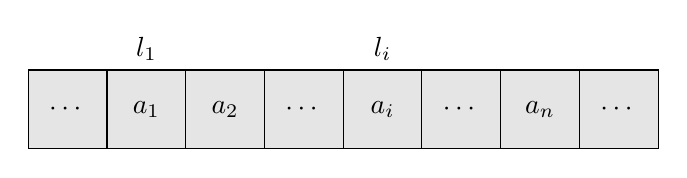
\begin{tikzpicture}
\foreach \i in {1,...,8}
\filldraw[fill=black!10] (\i-1,0)rectangle(\i,1);
\node [] at (0.5,0.5) {$\cd$};
\node [] at (1.5,0.5) {$a_1$}; \node [above] at (1.5,1) {$l_1$}; 
\node [] at (2.5,0.5) {$a_2$};
\node [] at (3.5,0.5) {$\cd$};
\node [] at (4.5,0.5) {$a_i$}; \node [above] at (4.5,1) {$l_i$}; 
\node [] at (5.5,0.5) {$\cd$};
\node [] at (6.5,0.5) {$a_n$};
\node [] at (7.5,0.5) {$\cd$};
\end{tikzpicture}
\caption{线性表的顺序存储}
\end{figure}


%第$i+1$个数据元素的存储位置$Loc(a_{i+1})$和第$i$个数据元素的存储位置$Loc(a_{i})$之间满足
$$
l(a_{i+1})=l(a_{i})+k
$$
%其中$l$为线性表每个元素需占用的存储单元. 特别地,  
$$
l(a_{i})=l(a_{1})+(i-1)k
$$
\end{frame}

\begin{frame}[fragile]\ft{\subsecname}
\begin{lstlisting}[title=顺序存储的结构代码,language=C,frame=tb,backgroundcolor=\color{red!10}]
#define MAX_SIZE 100
typedef int ElemType;
typedef struct sqlist {
    ElemType data[MAX_SIZE];
    int length;
} SqList;
\end{lstlisting}

\end{frame}

\subsection{顺序表的基本操作}
\begin{frame}\ft{\subsecname}
\begin{itemize}
\item
初始化
\item
赋值
\item
查找
\item
修改
\item
插入
\item
删除
\item
求长度
\item
$\cd$
\end{itemize}•
\end{frame}

\begin{frame}[fragile]\ft{初始化}
\begin{lstlisting} [language=C,frame=tb,backgroundcolor=\color{red!10}]
Status SqListInit(SqList *L) {
  L->data=(ElemType *) malloc(MAX_SIZE*sizeof(ElemType));
  if(!L->data) return ERROR;
  L->length=0;
  return OK;
}
\end{lstlisting}

\end{frame}

\begin{frame}[fragile]\ft{插入结点}
\begin{block}{目标}
在$L=(a_1,\cd,a_{i-1},\red{a_i},a_{i+1},\cd,a_n)$中的第$i$个位置上插入新结点$e$,  使其成为
$$
L=(a_1,\cd,a_{i-1},e,a_i,a_{i+1},\cd,a_n)
$$
\end{block}

\begin{block}{实现步骤}
\begin{itemize}
\item[(1)]
将第$i$个至第$n$个结点后移一个位置;
\item[(2)]
将结点$e$插入到结点$a_{i-1}$之后;
\item[(3)]
线性表长度加1.
\end{itemize}•
\end{block}

\end{frame}

\begin{frame}[fragile]\ft{插入结点}
\begin{lstlisting} [language=C,breaklines,backgroundcolor=\color{red!10},frame=tb]
Status SqListInsert(SqList *L,int i,ElemType e){
  int j;
  if (L->length>=MAX_SIZE) { //`线性表已满`
    printf("`线性表溢出!`\n"); return ERROR;
  }
  if (i<0||i>L->length-1)   //`i不在范围内`
    return ERROR;
  for (j=L->length-1; j>=i-1; j--)
    L->data[j+1]=L->data[j];
  L->data[i-1]=e;
  L->length++;
  return OK;
}
\end{lstlisting}

\end{frame}

\begin{frame}\ft{插入结点}
在$L$的第$i$个元素之前插入新结点,  其时间主要耗费在结点的移动上. 因此,  可用结点的移动来估计算法的时间复杂度. \vspace{0.1in}

设在$L$的第$i$个元素之前插入结点的概率为$p_i$. 不失一般性,  设各位置插入等概率,  则$p_i=\frac1{n+1}$,  而插入时移动结点的次数为$n-i+1$,  故总的平均移动次数为
$$
E_{insert}=\sum_{i=1}^n p_i (n-i+1)=\frac n2.
$$\vspace{0.1in}

这表明,  在顺序表上做插入运算,  平均要移动表上一半的结点. 当表长$n$较大时,  算法效率相当低. 因此算法的平均时间复杂度为$O(n)$. 
\end{frame}

\begin{frame}\ft{删除结点}
\begin{block}{目标}
在
$$
L=(a_1,\cd,a_{i-1},\red{a_i},a_{i+1},\cd,a_n)
$$
中删除结点$a_i$,  使其成为 
$$
L=(a_1,\cd,a_{i-1},a_{i+1},\cd,a_n)
$$
\end{block}

\begin{block}{实现步骤}
\begin{itemize}
\item[(1)]
将$L$中的第$i+1$个至第$n$个结点依次前移一个位置;
\item[(2)]
线性表长度减1.
\end{itemize}•
\end{block}
\end{frame}


\begin{frame}[fragile]\ft{删除结点}
\begin{lstlisting} [language=C]
Status SqListDelete(SqList * L, int i, ElemType * e) {
  int j; 
  if (L->length == 0){
    printf("List is empty!\n"); return ERROR;
  }
  if (i<0||i>L->length){
    printf("Element deleted does not exist!\n"); 
    return ERROR;
  }
  else {
    *e=L->data[i-1];
    for (j=i; j<L->length; j++)
      L->data[j-1]=L->data[j];
    L->length--;
    return OK;
  }
}
\end{lstlisting}

\end{frame}


\begin{frame}\ft{删除结点}
删除$L$的第$i$个元素,  其时间主要耗费在表中结点的移动操作上. 因此,  可用结点的移动来估计算法的时间复杂度. \vspace{0.1in}

设在$L$中删除第$i$个元素的概率为$p_i$,  不失一般性,  设各个位置插入等概率,  则$p_i=\frac1{n}$,  而插入时移动结点的次数为$n-i$,  故总的平均移动次数为
$$
E_{delete}=\sum_{i=1}^n p_i (n-i)=\frac {n-1}2.
$$\vspace{0.1in}

这表明,  在顺序表上做删除运算,  平均要移动表上一半的结点. 当表长$n$较大时,  算法效率相当低. 因此算法的平均时间复杂度为$O(n)$. 
\end{frame}

\begin{frame}\ft{查找、定位删除}
\begin{block}{目标}
在$L=(a_1,a_2,\cd,a_n)$中删除值为$x$的第一个结点. 
\end{block}

\begin{block}{实现步骤}
\begin{itemize}
\item[(1)]
在$L$中查找值为$x$的第一个数据元素;
\item[(2)]
将从找到的位置至最后一个结点依次向前移动一个位置;
\item[(3)]
线性表长度减1. 
\end{itemize}
\end{block}
\end{frame}


\begin{frame}[fragile]\ft{查找、定位删除}
\begin{lstlisting} [language=C,breaklines,backgroundcolor=\color{red!10},frame=tb]
Status SqListLocateDelete(SqList *L,ElemType x) {
  int i=0,k;
  while (i<L->length){
    if (L->data[i]!=x) i++;
    else {
      for (k=i+1;k<L->length;k++)
        L->data[k-1]=L->data[k];
      L->length--; break;
    }
  }
  if (i>L->length) {
    printf("要删除的数据元素不存在!\n");
    return ERROR;
  }
  return OK;
}
\end{lstlisting}

\end{frame}

\begin{frame}\ft{查找、定位删除}
时间主要耗费在数据元素的比较和移动操作上. \vspace{0.1in}

 
设在$L$中删除数据元素的概率为$p_i$,  不失一般性,  设各个位置等概率,  则$p_i=\frac1{n}$. 
\begin{itemize}
\item 比较的平均次数为:
$$
E_{compare} = \sum_{i=1}^n p_i i= \frac{n+1}2
$$
\item 删除时的平均移动次数为
$$
E_{delete} =\sum_{i=1}^n p_i (n-i)=\frac {n-1}2.
$$\
\end{itemize}•
平均时间复杂度为
\[
E_{compare}+E_{delete}=n
\]

\end{frame}



 %%%%%%%%%%%%%%%%%%%%
\subsection{线性表的链式存储}
\begin{frame}\ft{\subsecname}
\begin{dingyi}[链式存储]
用一组任意的存储单元存储线性表中的数据元素。
用这种方法存储的线性表简称\textcolor{acolor3}{链表}。
\end{dingyi}

\pause 
\begin{itemize}
\item 
在链表中,结点的存储单元可以连续,也可以不连续,甚至可以零散地分布在内存中的任意位置。
\item 
链表的逻辑顺序和物理顺序不一定相同。
\end{itemize} 
\end{frame}


\begin{frame}\ft{链表}
\begin{figure}
\centering
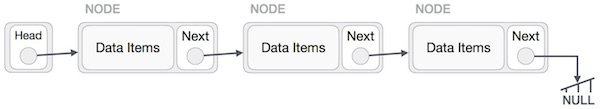
\includegraphics[width=4.5in]{Chapters/Ch02/Fig/linked_list.jpg}
\end{figure}

\begin{figure}
\centering
\begin{tikzpicture}
\foreach \i in {1,2}
\filldraw[very thick,fill=black!10] (\i-1,0)rectangle(\i,1);
\node [] at (0.5,0.5) {data};
\node [] at (1.5,0.5) {next};
\node [right] at (3.5,1) {data: 数据域,存放结点的值};
\node [right] at (3.5,0.2) {next: 指针域,存放结点的直接后继的地址};
\end{tikzpicture}
\end{figure}

\end{frame}

\begin{frame}\ft{链表}
\begin{itemize}
\item 
链表是通过每个结点的指针域将线性表的$n$个结点按其逻辑次序链接在一起的。
\item 
每一个结点只包含一个指针域的链表,称为单链表。
\item 
为操作方便,总在链表的第一个结点之前附设一个头结点(头指针)head指向第一个结点。头结点的数据域可以不存储任何信息(或链表长度等信息)。
\item 
单链表由表头唯一确定,因此单链表可用头指针的名字来命名。
\end{itemize}
\end{frame}

\begin{frame}\ft{链表}
\begin{figure}
\centering
\begin{tikzpicture}
\node [right] at (0,6.5) {例1:线性表$L=(bat,cat,eat,fat,hat)$};

\pause 

\foreach \i in {1,4,7} {
\filldraw[thick,fill=red!20,rounded corners] (\i-1,2)rectangle(\i+1,3);
\draw[thick](\i-1+1.33,2)--(\i-1+1.33,3);
\filldraw[thick,fill=red!20,rounded corners] (\i-1,0.5)rectangle(\i+1,1.5);
\draw[thick](\i-1+1.33,.5)--(\i-1+1.33,1.5);
}
\foreach \i in {1,4} {
\draw[thick,->] (\i-1+1.67,2.5)--(\i+2,2.5);
\draw[thick,->] (\i-1+1.67,1)--(\i+2,1);
}

\draw[thick,->] (6+1.67,2.5)--(6+2.3,2.5)--(6+2.3,1.75)--(0.67,1.75)--(0.67,1.5);
\draw[thick,->] (6+1.67,1)--(6+2.5,1)--(6+2.5,0.5);
\draw[thick] (6+2.2,0.4)--(6+2.5,0.5)--(6+2.8,.6);
\draw[thick] (6+2.2,0.4)--(6+2.2,0.3);
\draw[thick] (6+2.5,0.5)--(6+2.5,0.3);
\draw[thick] (6+2.8,0.6)--(6+2.8,0.3);

\node [above] at (0.6,3) {head};
\node [] at (3+0.6,2.5) {bat};
\node [] at (6+0.6,2.5) {cat};
\node [] at (0.6,1) {eat};
\node [] at (3+0.6,1) {fat};
\node [] at (6+0.6,1) {hat};

\pause 

\foreach \i in {1,2,...,14} {
\filldraw[fill=blue!20] (10,\i*0.5-0.5)rectangle(11.5,\i*0.5);
}
\node [] at (10.75,6.75) {$\cd$};
\node [] at (10.75,6.25) {hat};         
\node [left] at (10,6.25) {$1100$};
\node [] at (10.75,5.75) {null};
\node [] at (10.75,5.25) {$\cd$};
\node [] at (10.75,4.75) {cat};        
\node [left] at (10,4.75) {$1300$};
\node [] at (10.75,4.25) {$1305$};
\node [] at (10.75,3.75) {eat};     \node [left] at (10,3.75) {1305};
\node [] at (10.75,3.25) {$3700$};
\node [] at (10.75,2.75) {$\cd$};
\node [] at (10.75,2.25) {bat};
\node [] at (10.75,1.75) {$1300$};
\node [] at (10.75,1.25) {fat};    
\node [left] at (10,1.25) {$3700$};
\node [] at (10.75,0.75) {$1100$};
\node [] at (10.75,0.25) {$\cd$};
\end{tikzpicture}
\end{figure}
\end{frame}
%
%
\begin{frame}[fragile]\ft{链表}
\textcolor{acolor5}{结点的描述与实现}
\lstinputlisting
[title=LinkList.h,language=C,linerange={11-16}]
{Chapters/Ch02/Code/LinkList/LinkList.h}
\end{frame}
%
\begin{frame}[fragile]\ft{\subsecname}
\textcolor{acolor5}{结点的实现}
结点是通过动态分配和释放来实现的,即需要时分配,不需要时释放。
\begin{lstlisting}[frame=no]
malloc(), realloc(), sizeof(), free();
\end{lstlisting}
\pause 
\begin{itemize}
\item 动态分配
\begin{lstlisting}[frame=no]
p = (LNode *) malloc(sizeof(LNode));
\end{lstlisting}
分配了一个类型为$LNode$的结点变量的空间,并将其首地址放入指针变量$p$中。\\[0.1in]
\item \pause 动态释放
\begin{lstlisting}[frame=no]
free(p);
\end{lstlisting}
系统回收由指针变量$p$指向的内存区。
\end{itemize}
\end{frame}
%
\begin{frame}[fragile]\ft{链表常用操作}
\begin{itemize}
\item[(1)] 结点的赋值
\begin{figure}
\centering
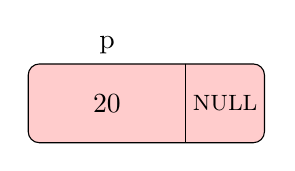
\begin{tikzpicture}
  \filldraw[fill=red!20,rounded corners](0,0)rectangle(3,1); 
  \node [] at (1,0.5) {20};
  \draw(2,0)rectangle(2,1); 
  \node [] at (2.5,0.5) {\footnotesize NULL};
  \node [above] at (1,1) {p};
\end{tikzpicture}
\end{figure}

\begin{figure}
\centering
\begin{tikzpicture}
  \filldraw[fill=red!20,rounded corners](0,0)rectangle(3,1); 
  \node [] at (1,0.5) {20};
  \draw(2,0)rectangle(2,1); 
  \node [] at (2.5,0.5) {\footnotesize NULL};
  \node [above] at (1,1) {p};
\end{tikzpicture}
\end{figure}

\end{itemize}

\end{frame}
%
%
\begin{frame}[fragile]\ft{链表常用操作}
\begin{itemize}
\item[(2)] 常见的指针操作
\begin{figure}
\centering
\begin{tikzpicture}[scale=1.5]
\def \x{0.5}
\foreach \d in {0,4}{
\filldraw[fill=red!20,rounded corners](\d+0,0)rectangle(\d+2*\x,\x);  
\draw (\d+1.33*\x,0)rectangle(\d+1.33*\x,\x);  
\node [] at (\d+0.67*\x,0.5*\x) {a};
\node [above] at (\d+0.67*\x,2*\x) {p};
\draw[->,line width=1.5pt](\d+0.67*\x,2*\x)--(\d+0.67*\x,1.1*\x);
\draw[->,line width=1.5pt](\d-1*\x,0.5*\x)--(\d+0*\x,0.5*\x);
\draw[->,line width=1.5pt](\d+1.5*\x,0.5*\x)--(\d+2.5*\x,0.5*\x);
}

\def \d{4}
\node[below] at (\x,0) {操作前};
\node[below] at (\d+\x,0) {操作后};
\node [above] at (\d-\x,2*\x) {q};
\draw[->,line width=1.5pt] (\d-1*\x,2*\x)--(\d-1*\x,\x)--(\d+0*\x,\x);

\end{tikzpicture}
\caption{q=p}
\end{figure}
\end{itemize}
\end{frame}
%
%
\begin{frame}[fragile]\ft{链表常用操作} 
\begin{figure}
\centering
\begin{tikzpicture}[scale=1.5]
\def \x{0.5}
\foreach \d in {0,4}{
\filldraw[fill=red!20,rounded corners](\d+0,0)rectangle(\d+2*\x,\x);  
\draw (\d+1.33*\x,0)--(\d+1.33*\x,\x); 
\filldraw[fill=red!20,rounded corners](\d+3*\x,0)rectangle(\d+5*\x,\x);  
\draw (\d+3*\x+1.67*\x,0)--(\d+3*\x+1.67*\x,\x); 

 
\node [] at (\d+0.67*\x,0.5*\x) {a};
\node [] at (\d+3.67*\x,0.5*\x) {b};
\node [above] at (\d+0.67*\x,2*\x) {p};
\draw[->,line width=1.5pt](\d+0.67*\x,2*\x)--(\d+0.67*\x,1.1*\x);
\draw[->,line width=1.5pt](\d-1*\x,0.5*\x)--(\d+0*\x,0.5*\x);
\draw[->,line width=1.5pt](\d+1.5*\x,0.5*\x)--(\d+3*\x,0.5*\x);
}

\def \d{4}
\node[below=4pt] (before) at (3*\x,0) {操作前};
\node[below=4pt] (after) at (\d+3*\x,0) {操作后};
\node [above] at (\d+3.67*\x,2*\x) {q};
\draw[->,line width=1.5pt] (\d+3.67*\x,2*\x)--(\d+3.67*\x,1.1*\x);
\end{tikzpicture}
\caption{q = p->next}
\end{figure}
\end{frame}

\begin{frame}[fragile]\ft{链表常用操作}
\begin{figure}
\centering
\begin{tikzpicture}
\def \x{0.5}
\foreach \d in {0,5}{
\filldraw[fill=red!20](\d+0,0)rectangle(\d+\x,\x);  
\filldraw[fill=red!20](\d+\x,0)rectangle(\d+2*\x,\x); 
\filldraw[fill=red!20](\d+3*\x,0)rectangle(\d+4*\x,\x);  
\filldraw[fill=red!20](\d+4*\x,0)rectangle(\d+5*\x,\x); 

\node [] at (\d+0.5*\x,0.5*\x) {a};
\node [] at (\d+3.5*\x,0.5*\x) {b};

\draw[->](\d-1*\x,0.5*\x)--(\d+0*\x,0.5*\x);
\draw[->](\d+1.5*\x,0.5*\x)--(\d+3*\x,0.5*\x);
}
\def\d{0}
\draw[->](\d+0.5*\x,2*\x)--(\d+0.5*\x,\x);
\node [above] at (\d+0.5*\x,2*\x) {p};


\def \d{5}
\node[below] at (3*\x,0) {操作前};
\node[below] at (\d+3*\x,0) {操作后};
\node [above] at (\d+3.5*\x,2*\x) {p};
\draw[->] (\d+3.5*\x,2*\x)--(\d+3.5*\x,\x);
\end{tikzpicture}
\caption{p=p-\textgreater next;}
\end{figure}
\end{frame}

\begin{frame}[fragile]\ft{链表常用操作} 
\begin{figure}
\centering

\begin{tikzpicture}
\def \x{0.5}

\foreach \d in {0,5}{
\filldraw[fill=red!20](\d+0,0)rectangle(\d+\x,\x);  
\filldraw[fill=red!20](\d+\x,0)rectangle(\d+2*\x,\x); 
\filldraw[fill=red!20](\d+3*\x,0)rectangle(\d+4*\x,\x);  
\filldraw[fill=red!20](\d+4*\x,0)rectangle(\d+5*\x,\x); 
\filldraw[fill=red!20](\d+3*\x,-1.5*\x)rectangle(\d+4*\x,-0.5*\x);  
\filldraw[fill=red!20](\d+4*\x,-1.5*\x)rectangle(\d+5*\x,-0.5*\x); 

 
\node [] at (\d+0.5*\x,0.5*\x) {a};
\node [] at (\d+3.5*\x,0.5*\x) {b};
\node [] at (\d+3.5*\x,-1*\x) {c};
\node [left] at (\d+1.5*\x,-1*\x) {p};

\draw[->](\d-1*\x,0.5*\x)--(\d+0*\x,0.5*\x);
\draw[->](\d+1.5*\x,-1*\x)--(\d+3*\x,-1*\x);

\draw[->](\d+0.5*\x,2*\x)--(\d+0.5*\x,\x);
\node [above] at (\d+0.5*\x,2*\x) {q};
}

\def\d{0}
\draw[->](\d+1.5*\x,0.5*\x)--(\d+3*\x,0.5*\x);
 
\def\d{5}
\draw[->](\d+1.5*\x,0.5*\x)--(\d+2.5*\x,0.5*\x)--(\d+2.5*\x,-0.5*\x)--(\d+3*\x,-0.5*\x);

\def \d{5}
\node[below] at (3*\x,-1.5*\x) {操作前};
\node[below] at (\d+3*\x,-1.5*\x) {操作后};
%\node [above] at (\d+3.5*\x,2*\x) {q};
%\draw[->] (\d+3.5*\x,2*\x)--(\d+3.5*\x,\x);

\end{tikzpicture}
\caption{q-\textgreater next=p;}
\end{figure}
\end{frame}


\begin{frame}[fragile]\ft{链表常用操作}
\begin{figure}
\centering

\begin{tikzpicture}
\def \x{0.5}

\foreach \c in {0,-2.5}{
\foreach \d in {0,5}{
\filldraw[fill=red!20](\d+0,\c+0)rectangle(\d+\x,\c+\x);  
\filldraw[fill=red!20](\d+\x,\c+0)rectangle(\d+2*\x,\c+\x); 
\filldraw[fill=red!20](\d+3*\x,\c+0)rectangle(\d+4*\x,\c+\x);  
\filldraw[fill=red!20](\d+4*\x,\c+0)rectangle(\d+5*\x,\c+\x); 

 
\draw[->](\d-1*\x,\c+0.5*\x)--(\d+0*\x,\c+0.5*\x);

\ifthenelse{  0 = \d \AND   -2 = \c}{
\draw[->](\d+1.5*\x,\c+0.5*\x)--(\d+1.5*\x,\c-0.5*\x)
--(5+0.5*\x,\c-0.5*\x)--(5+0.5*\x,\c);
}{
\draw[->](\d+1.5*\x,\c+0.5*\x)--(\d+3*\x,\c+0.5*\x);
}

\draw[->](\d+4.5*\x,\c+0.5*\x)--(\d+5.5*\x,\c+0.5*\x);
}
\node [] at (3.7,\c+0.5*\x) {$\cd\cd$};


\def\d{0}
\node [] at (\d+0.5*\x,\c+0.5*\x) {a};
\node [] at (\d+3.5*\x,\c+0.5*\x) {b};

\draw[->](\d+0.5*\x,\c+2*\x)--(\d+0.5*\x,\c+\x);
\node [above] at (\d+0.5*\x,\c+2*\x) {q};

\def\d{5}
\node [] at (\d+0.5*\x,\c+0.5*\x) {x};
\node [] at (\d+3.5*\x,\c+0.5*\x) {y};


\def \d{5}
\ifthenelse{  0 = \c}{
\node[below] at (7*\x,\c+0) {操作前};
}{
\node[below] at (7*\x,\c-1*\x) {操作后};
}

\node [above] at (\d+0.5*\x,\c+2*\x) {p};
\draw[->] (\d+0.5*\x,\c+2*\x)--(\d+0.5*\x,\c+\x);
}
\end{tikzpicture}
\caption{q-\textgreater next=p;}
\end{figure}
 
\end{frame}

%\begin{frame}[fragile]\ft{链表常用操作}
%\begin{figure}
\centering

\begin{tikzpicture}
\def \x{0.5}

\foreach \d in {0,5}{
\foreach \c in {0,-1}{
\filldraw[fill=red!20](\d+0,\c+0)rectangle(\d+\x,\c+\x);  
\filldraw[fill=red!20](\d+\x,\c+0)rectangle(\d+2*\x,\c+\x); 
\filldraw[fill=red!20](\d+3*\x,\c+0)rectangle(\d+4*\x,\c+\x);  
\filldraw[fill=red!20](\d+4*\x,\c+0)rectangle(\d+5*\x,\c+\x); 
 
\ifthenelse{0 = \c}{
\node [] at (\d+0.5*\x,\c+0.5*\x) {a};
\node [] at (\d+3.5*\x,\c+0.5*\x) {b};
}{
\node [] at (\d+0.5*\x,\c+0.5*\x) {x};
\node [] at (\d+3.5*\x,\c+0.5*\x) {y};
}

\draw[->](\d-1*\x,\c+0.5*\x)--(\d+0*\x,\c+0.5*\x);
\draw[->](\d+4.5*\x,\c+0.5*\x)--(\d+5.5*\x,\c+0.5*\x);

\ifthenelse{0 = \c \AND 5 = \d}{
\draw[->](\d+1.5*\x,\c+0.5*\x)--(\d+2.5*\x,\c+0.5*\x)
--(\d+2.5*\x,\c-\x)--(\d+3*\x,\c-\x);
}{
\draw[->](\d+1.5*\x,\c+0.5*\x)--(\d+3*\x,\c+0.5*\x);
}

\ifthenelse{0 = \c}{
\draw[->](\d+0.5*\x,\c+2*\x)--(\d+0.5*\x,\c+\x);
\node [above] at (\d+0.5*\x,\c+2*\x) {q};
}{}

\ifthenelse{-1 = \c}{
\node [left] at (\d-\x,\c+0.5*\x) {p};
}{}

}
\ifthenelse{0 = \d}{
\node [below] at (\d+2.5*\x,-2*\x) {操作前};
}{
\node [below] at (\d+2.5*\x,-2*\x) {操作后};
}

}
\end{tikzpicture}
\caption{q-\textgreater next=p-\textgreater next;}
\end{figure} 
%\end{frame}%
%
%\begin{frame}[fragile]\ft{链表常用操作}
%\begin{figure}
\centering

\begin{tikzpicture}
\def \x{0.5}

\foreach \c in {0,-2.5}{
\foreach \d in {0,5}{
\filldraw[fill=red!20](\d+0,\c+0)rectangle(\d+\x,\c+\x);  
\filldraw[fill=red!20](\d+\x,\c+0)rectangle(\d+2*\x,\c+\x); 
\filldraw[fill=red!20](\d+3*\x,\c+0)rectangle(\d+4*\x,\c+\x);  
\filldraw[fill=red!20](\d+4*\x,\c+0)rectangle(\d+5*\x,\c+\x); 

 
\draw[->](\d-1*\x,\c+0.5*\x)--(\d+0*\x,\c+0.5*\x);

\ifthenelse{  0 = \d \AND   -2 = \c}{
\draw[->](\d+1.5*\x,\c+0.5*\x)--(\d+1.5*\x,\c-0.5*\x)
--(5+3.5*\x,\c-0.5*\x)--(5+3.5*\x,\c);
}{
\draw[->](\d+1.5*\x,\c+0.5*\x)--(\d+3*\x,\c+0.5*\x);
}

\draw[->](\d+4.5*\x,\c+0.5*\x)--(\d+5.5*\x,\c+0.5*\x);
}
\node [] at (3.7,\c+0.5*\x) {$\cd\cd$};


\def\d{0}
\node [] at (\d+0.5*\x,\c+0.5*\x) {a};
\node [] at (\d+3.5*\x,\c+0.5*\x) {b};

\draw[->](\d+0.5*\x,\c+2*\x)--(\d+0.5*\x,\c+\x);
\node [above] at (\d+0.5*\x,\c+2*\x) {q};

\def\d{5}
\node [] at (\d+0.5*\x,\c+0.5*\x) {x};
\node [] at (\d+3.5*\x,\c+0.5*\x) {y};


\def \d{5}
\ifthenelse{  0 = \c}{
\node[below] at (7*\x,\c+0) {操作前};
}{
\node[below] at (7*\x,\c-1*\x) {操作后};
}

\node [above] at (\d+0.5*\x,\c+2*\x) {p};
\draw[->] (\d+0.5*\x,\c+2*\x)--(\d+0.5*\x,\c+\x);
}
\end{tikzpicture}
\caption{q-\textgreater next=p-\textgreater next;}
\end{figure}
 
%\end{frame}


\begin{frame}\ft{单链表的整表创建}
\begin{itemize}
\item  顺序存储结构的创建,就是一个数组的初始化。而单链表则不同,它可以很散,是一个动态结构。
\item 对每个链表而言,它所占用空间的大小和位置不需要预先分配,可根据系统的情况和实际需求即时生成。
\end{itemize}

所以创建单链表的过程就是一个动态生成链表的过程,即从空表的初始状态起,一次建立各元素结点,并逐个插入链表。
\end{frame}
%
%
\begin{frame}\ft{单链表的整表创建} 
动态创建单链表的常用方法有 
\begin{itemize}
\item 
头插法
\item 
尾插法
\end{itemize}
\end{frame}
%
\begin{frame}\ft{单链表的整表创建:头插法}
\begin{itemize}
\item 声明一结点$p$和计数器变量$i$;
\item 初始化一空链表$L$;
\item 让$L$的头结点的指针指向$NULL$,即建立一个带头结点的单链表;
\item 循环
\begin{itemize}
\item 生成一个新结点赋值给$p$
\item 随机生成一个数赋给$p$的数据域$p->data$ 
\item 将$p$插入到头结点与前一新结点之间
\end{itemize}
\end{itemize}
\end{frame}
%
\begin{frame}[fragile]\ft{单链表的整表创建:头插法}

%% \begin{lstlisting}[language=C,frame=tb,backgroundcolor=\color{red!10}]
//`随机生成n个元素,建立带表头结点的单链表L`
void CreateLinkListHead(LinkList *L, int n){
  LinkList p;
  int i;
  srand(time(0));
  *L=(LinkList) malloc(sizeof(LNode));
  (*L)->next=NULL;
  LNode *head, *p;
  for(i=0;i<n;i++)
    p=(LinkList)malloc(sizeof(LNode));
    p->data=rand()%100+1;
    p->next=(*L)->next;
    (*L)->next=p;
}
\end{lstlisting}

\lstinputlisting[
title=CreateLinkListHead.c,
language=C,
linerange={3-6,8-15},
numbers=left,
firstnumber=auto,
]{Chapters/Ch02/Code/LinkList/CreateLinkListHead.c}
\end{frame}

\begin{frame}\ft{单链表的整表创建:尾插法}
头插入法建立链表虽然算法简单,但生成的链表中结点的次序和输入的顺序相反。若希望二者次序一致,可采用尾插法建表。该方法是将新结点插入到当前链表的表尾,使其成为当前链表的尾结点。
\end{frame}
%
\begin{frame}\ft{单链表的整表创建:尾插法}
\lstinputlisting[
language=C,
linerange={3-6,8-17},
numbers=left,
firstnumber=auto,
]{Chapters/Ch02/Code/LinkList/CreateLinkListTail.c}
\end{frame}

\begin{frame}\ft{单链表的查找}
\begin{enumerate}
\item 按序号查找
\item 按值查找
\end{enumerate}
\end{frame}
%
\begin{frame}\ft{单链表的查找:按序号}


对于单链表,不能像顺序表中那样直接按序号$i$访问结点,而只能从链表的头结点出发,沿指针域next逐个结点往下搜索,知道搜到第$i$个结点为止。因此,链表不是随机存储结构。

\vspace{0.2in}

设单链表长度为$n$,要查找第$i$个结点,仅当$1\le i \le n$时,$i$的值是合法的。

\end{frame}
%
\begin{frame}[fragile]\ft{单链表的查找:按序号}
\lstinputlisting[
title=GetElem.c,
language=C,
linerange={3-13},
numbers=left,
firstnumber=auto,
]{Chapters/Ch02/Code/LinkList/GetElem.c}
\end{frame}

\begin{frame}[fragile]\ft{单链表的查找:按序号}
\lstinputlisting[
title=GetElem.c,
language=C,
linerange={15-21},
numbers=left,
firstnumber=12,
]{Chapters/Ch02/Code/LinkList/GetElem.c}
\end{frame}
%
\begin{frame}[fragile]\ft{单链表的查找:按序号}

\textcolor{acolor5}{移动指针$p$的频度:}
\[\left\{
\begin{array}{rl}
0\mbox{次},& i<1;\\[0.1in]
i-1\mbox{次}, & i  \in [1,n];\\[0.1in]
n\mbox{次}, & i>n.
\end{array}
\right.
~~\Rightarrow~~\mbox{时间复杂度为}O(n).
\] 

\end{frame}


\begin{frame}\ft{单链表的查找:按值}

按值查找是在链表中,查找是否有结点值等于给定值$key$的结点?
\begin{itemize}
\item
若有,则返回首次找到的值为$key$的结点的存储位置;
\item
否则返回$NULL$。
\end{itemize}
查找时从开始结点出发,沿链表逐个将结点的值和给定值$key$作比较。

\end{frame}

\begin{frame}[fragile]\ft{单链表的查找:按值}
\lstinputlisting[
title=LocateNodeKey.c,
language=C,
linerange={3-14},
numbers=left,
firstnumber=auto,
]{Chapters/Ch02/Code/LinkList/LocateNodeKey.c}

\end{frame}

\begin{frame}[fragile]\ft{单链表的查找:按值}

\textcolor{acolor5}{平均时间复杂度:}
算法的执行与形参$key$有关,平均时间复杂度为$O(n)$。

\end{frame}

\begin{frame}\ft{单链表中插入结点}

插入运算是指将值为$e$的新结点插入到表的第$i$个结点的位置上,即插入到$a_{i-1}$与$a_i$之间。因此,必须首先找到$a_{i-1}$所在的结点$p$,然后生成一个数据域为$e$的新结点$q$,$q$作为$p$的直接后继。
\end{frame}

\begin{frame}\ft{单链表中插入结点}
\begin{figure}
\centering
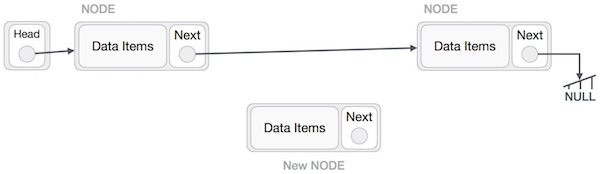
\includegraphics[width=4.5in]{Chapters/Ch02/Fig/linked_list_insertion_0.jpg}\\[0.1cm]\pause 
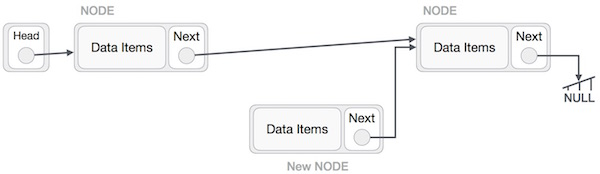
\includegraphics[width=4.5in]{Chapters/Ch02/Fig/linked_list_insertion_1.jpg}
\end{figure}
\end{frame}

\begin{frame}\ft{单链表中插入结点}
\begin{figure}
\centering
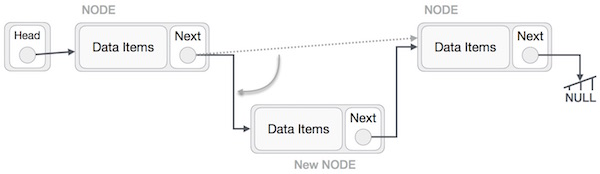
\includegraphics[width=4.5in]{Chapters/Ch02/Fig/linked_list_insertion_2.jpg}\\[0.1cm]\pause 
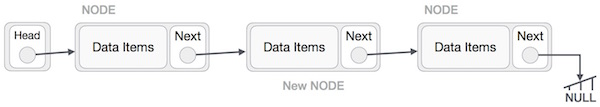
\includegraphics[width=4.5in]{Chapters/Ch02/Fig/linked_list_insertion_3.jpg}
\end{figure}
\end{frame}

\begin{frame}\ft{单链表中插入结点}
\lstinputlisting[
title=InsertLNode.c,
language=C,
linerange={3-12},
numbers=left,
firstnumber=auto,
]{Chapters/Ch02/Code/LinkList/InsertLNode.c}
\end{frame}

\begin{frame}\ft{单链表中插入结点}
\lstinputlisting[
title=InsertLNode.c,
language=C,
linerange={14-23},
numbers=left,
firstnumber=11,
]{Chapters/Ch02/Code/LinkList/InsertLNode.c}
\end{frame}
%
%
\begin{frame}\ft{单链表中插入结点}

\textcolor{acolor5}{平均时间复杂度:}
设链表长度为$n$,合法的插入位置是$1\le i \le n$。
算法的时间主要耗费在移动指针$p$上,平均时间复杂度为$O(n)$。

\end{frame}
 
 
\begin{frame}\ft{单链表中删除结点}
\begin{itemize}
\item 
按序号删除:删除单链表中的第$i$个结点。\\[0.2in]
\item 
按值删除:删除单链表中值为$key$的第一个结点。
\end{itemize}
\end{frame}
 
 
\begin{frame}\ft{单链表中删除结点}
\begin{figure}
\centering
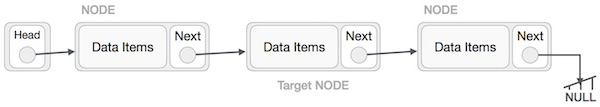
\includegraphics[width=4.5in]{Chapters/Ch02/Fig/linked_list_deletion_0.jpg}\\[0.1cm]\pause 
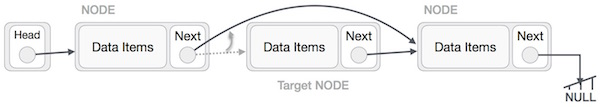
\includegraphics[width=4.5in]{Chapters/Ch02/Fig/linked_list_deletion_1.jpg}\\[0.1cm]\pause 
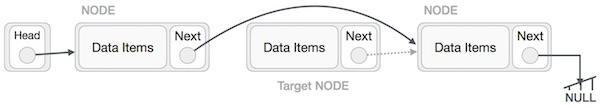
\includegraphics[width=4.5in]{Chapters/Ch02/Fig/linked_list_deletion_2.jpg}
\end{figure}
\end{frame}


\begin{frame}\ft{单链表中删除结点:按序号}
\begin{itemize}
\item 为了删除第$i$个结点$a_i$,必须找到结点的存储地址;
\item 该存储地址在其直接前驱结点$a_{i-1}$的$next$域中,因此必须首先找到$a_{i-1}$的存储位置$p$,
然后令$p$->$next$指向$a_i$的直接后继结点,即把$a_i$从链上摘下来。
\item
最后释放结点$a_i$的空间,将其归还给“存储池”。
\end{itemize}•

\end{frame}


\begin{frame}\ft{单链表中删除结点:按序号}
设单链表长度为$n$,则删去第$i$个结点仅当$1\le i \le n$时是合法的。当$i=n+1$时,虽然被删结点不存在,但其前驱结点却存在,是终端结点。故判断条件之一是$p$->$next!=NULL$。

\end{frame}

\begin{frame}[fragile]\ft{单链表中删除结点:按序号}
\lstinputlisting[
title=DeleteLNodeIndex.c,
language=C,
linerange={3-6},
numbers=left,
firstnumber=auto,
]{Chapters/Ch02/Code/LinkList/DeleteLNodeIndex.c}
\end{frame}

\begin{frame}[fragile]\ft{单链表中删除结点:按序号}
\lstinputlisting[
title=DeleteLNodeIndex.c,
language=C,
linerange={8-15},
numbers=left,
firstnumber=5,
]{Chapters/Ch02/Code/LinkList/DeleteLNodeIndex.c}
\end{frame}

\begin{frame}[fragile]\ft{单链表中删除结点:按序号}
\lstinputlisting[
title=DeleteLNodeIndex.c,
language=C,
linerange={17-24},
numbers=left,
firstnumber=13,
]{Chapters/Ch02/Code/LinkList/DeleteLNodeIndex.c}
\end{frame}

\begin{frame}[fragile]\ft{单链表中删除结点:按序号}
\textcolor{acolor5}{时间复杂度:}
时间复杂度为$O(n)$。
 

\end{frame}


\begin{frame}\ft{单链表中删除结点:按值}

与按值查找相类似,首先要查找值为$key$的结点是否存在?
\begin{itemize}
\item 若存在,则删除;
\item 否则返回$NULL$。
\end{itemize}

\end{frame}

\begin{frame}[fragile]\ft{单链表中删除结点:按值}
\lstinputlisting[
title=DeleteLNodeKey.c,
language=C,
linerange={3-11},
numbers=left,
firstnumber=auto,
]{Chapters/Ch02/Code/LinkList/DeleteLNodeKey.c}
\end{frame}

\begin{frame}[fragile]\ft{单链表中删除结点:按值}
\lstinputlisting[
title=DeleteLNodeKey.c,
language=C,
linerange={12-24},
numbers=left,
firstnumber=10,
]{Chapters/Ch02/Code/LinkList/DeleteLNodeKey.c}
\end{frame}
%
\begin{frame}[fragile]\ft{单链表中删除结点:按值}

\textcolor{acolor5}{时间复杂度}
时间复杂度为$O(n)$。
\end{frame}

\begin{frame}[fragile]\ft{单链表中删除结点}
链表实现插入和删除运算,无需移动结点,仅需修改指针,解决了顺序表的插入或删除操作需要移动大量元素的问题。
\end{frame}

\begin{frame}[fragile]\ft{单链表中删除多个结点:按值}
\begin{wenti}
删除单链表中值为$key$的所有结点。
\end{wenti}
\pause 
\textcolor{acolor5}{基本思想}
\begin{itemize}
\item
从单链表的第一个结点开始,对每个结点进行检查,若结点的值为$key$,则删除之;
\item
然后检查下一个结点,直到所有的结点都检查。
\end{itemize}

\end{frame}

\begin{frame}[fragile]\ft{单链表中删除多个结点:按值}
\lstinputlisting[
title=DeleteLNodesKey.c,
language=C,
linerange={3-13},
numbers=left,
firstnumber=auto,
]{Chapters/Ch02/Code/LinkList/DeleteLNodesKey.c}
\end{frame}

\begin{frame}[fragile]\ft{单链表中删除多个结点:按值}
\lstinputlisting[
title=DeleteLNodesKey.c,
language=C,
linerange={14-20},
numbers=left,
firstnumber=12,
]{Chapters/Ch02/Code/LinkList/DeleteLNodesKey.c}
\end{frame}



\begin{frame}[fragile]\ft{单链表中删除重复结点}
\begin{wenti}
删除单链表中所有值重复的结点,使得所有结点的值都不相同。
\end{wenti}
\pause 
\textcolor{acolor5}{基本思想}
从单链表的第一个结点开始,对每个结点进行检查:
\begin{itemize}
\item
检查链表中该结点的所有后继结点,只要有值和该结点的值相同,则删除之;
\item
然后检查下一个结点,直到所有的结点都检查。
\end{itemize}
\end{frame}



\begin{frame}[fragile]\ft{单链表中删除重复结点}
\lstinputlisting[
title=DeleteDupLNodes.c,
language=C,
linerange={3-9},
numbers=left,
firstnumber=auto,
]{Chapters/Ch02/Code/LinkList/DeleteDupLNodes.c}
\end{frame}

\begin{frame}[fragile]\ft{单链表中删除重复结点}
\lstinputlisting[
title=DeleteDupLNodes.c,
language=C,
linerange={10-17},
numbers=left,
firstnumber=8,
]{Chapters/Ch02/Code/LinkList/DeleteDupLNodes.c}
\end{frame}

\begin{frame}[fragile]\ft{单链表中删除重复结点}
\lstinputlisting[
title=DeleteDupLNodes.c,
language=C,
linerange={18-26},
numbers=left,
firstnumber=16,
]{Chapters/Ch02/Code/LinkList/DeleteDupLNodes.c}
\end{frame}

%\begin{frame}[fragile]\ft{单链表的逆转}
%\begin{figure}
%\centering
%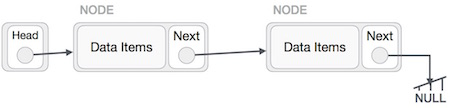
\includegraphics[width=4.5in,height=.8in]{Chapters/Ch02/Fig/linked_list_reverse_0.jpg}\\[0.1cm]\pause 
%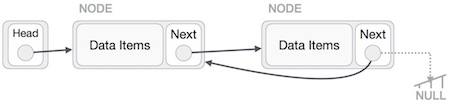
\includegraphics[width=4.5in,height=.8in]{Chapters/Ch02/Fig/linked_list_reverse_1.jpg}\\[0.1cm]\pause 
%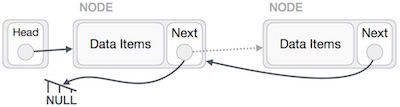
\includegraphics[width=4.5in,height=.8in]{Chapters/Ch02/Fig/linked_list_reverse_2.jpg}
%\end{figure}
%\end{frame}
%
%\begin{frame}[fragile]\ft{单链表的逆转}
%\begin{figure}
%\centering 
%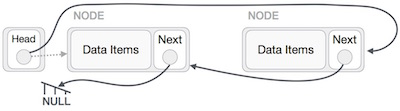
\includegraphics[width=4.5in,height=.8in]{Chapters/Ch02/Fig/linked_list_reverse_3.jpg} 
%\end{figure}
%\end{frame}
 

\begin{frame}\ft{单链表的合并}
设有两个有序的单链表,它们的头指针分别为$La$、$Lb$,
将它们合并为以$Lc$为头指针的有序链表。 
\begin{figure}
\centering
\begin{tikzpicture}[scale=0.9]
\def \x{1}
\def \y{0.6}

\foreach \c in {0,-2}{
\foreach \d in {0,2,4,6,8,10}{
\ifthenelse{  8 = \d }{
\node[left] at (\d+\x,\c+0.5*\y) {$\cd$};
}{
\filldraw[fill=red!20](\d+0,\c+0)rectangle(\d+\x,\c+\y);  
\filldraw[fill=red!20](\d+\x,\c+0)rectangle(\d+1.3*\x,\c+\y); 
}
\ifthenelse{  10 = \d}{

}{\draw[->,>=stealth] (\d+1.15*\x,\c+0.5*\y)--(\d+1.95*\x,\c+0.5*\y);}

\ifthenelse{ 0 = \c }{
\node[]at( 2.5,\c+0.5*\y){$-7$};
\node[]at( 4.5,\c+0.5*\y){$3$}; 
\node[]at( 6.5,\c+0.5*\y){$12$};
\node[]at(10.5,\c+0.5*\y){$23$};
\draw[->,>=stealth] (-.5*\x,\c+0.2*\y) node [left] {$Lc$}--(-0.1*\x,\c+0.2*\y);
\draw[->,>=stealth] (-.5,\c+0.8*\y) node[left] {$pc$}--(-.1*\x,\c+0.8*\y);
\draw[->,>=stealth] (2.5,\c+1.5*\y) node[above] {$pa$}--(2.5,\c+1.1*\y);
\draw[->,>=stealth] (0.5,\c+1.5*\y)node[above] {$La$} --(0.5,\c+1.1*\y);
}{
\node[]at( 2.5,\c+0.5*\y){$-2$};
\node[]at( 4.5,\c+0.5*\y){$4$}; 
\node[]at( 6.5,\c+0.5*\y){$9$};
\node[]at(10.5,\c+0.5*\y){$15$};
\draw[->,>=stealth] (2.5,\c-0.5*\y) node[below] {$pb$}--(2.5,\c-0.1*\y);
\draw[->,>=stealth] (0.5,\c-0.5*\y) node[below] {$Lb$}--(0.5,\c-0.1*\y);
}
}
}
\end{tikzpicture}
\caption{合并前的示意图}
\end{figure} 
\end{frame}


\begin{frame}\ft{单链表的合并}
\begin{figure}
\centering
\begin{tikzpicture}[scale=0.9]
\def \x{1}
\def \y{0.6}

\foreach \c in {0,-2}{
\foreach \d in {0,2,4,6,8,10}{
\ifthenelse{  8 = \d }{
\node[left] at (\d+\x,\c+0.5*\y) {$\cd$};
}{
\filldraw[fill=red!20](\d+0,\c+0)rectangle(\d+\x,\c+\y);  
\filldraw[fill=red!20](\d+\x,\c+0)rectangle(\d+1.3*\x,\c+\y); 
}
\ifthenelse{   2 = \d \AND   0 = \c \OR  0 = \d \AND   0 = \c \OR 10 = \d}{

}{\draw[->,>=stealth] (\d+1.15*\x,\c+0.5*\y)--(\d+1.95*\x,\c+0.5*\y);}

\ifthenelse{ 0 = \c }{
\node[]at( 2.5,\c+0.5*\y){$-7$};
\node[]at( 4.5,\c+0.5*\y){$3$}; 
\node[]at( 6.5,\c+0.5*\y){$12$};
\node[]at(10.5,\c+0.5*\y){$23$};
\draw[->,>=stealth] (4.5,\c+1.5*\y) node[above] {$pa$}--(4.5,\c+1.1*\y);
\draw[->,>=stealth] (0.5,\c+1.5*\y)node[above] {$La$} --(0.5,\c+1.1*\y);
}{
\node[]at( 2.5,\c+0.5*\y){$-2$};
\node[]at( 4.5,\c+0.5*\y){$4$}; 
\node[]at( 6.5,\c+0.5*\y){$9$};
\node[]at(10.5,\c+0.5*\y){$15$};
\draw[->,>=stealth] (4.5,\c-0.5*\y) node[below] {$pb$}--(4.5,\c-0.1*\y);
\draw[->,>=stealth] (2.5,\c-0.5*\y) node[below] {$pc$}--(2.5,\c-0.1*\y);
\draw[->,>=stealth] (0.5,\c-0.5*\y) node[below] {$Lb$}--(0.5,\c-0.1*\y);
}

\ifthenelse{ 0 = \c }{
\draw[->,>=stealth,red] (-.5*\x,\c+0.5*\y) node [left] {$Lc$}--(-0.1,\c+0.5*\y);
\draw[->,>=stealth,red] (0+1.15*\x,\c+0.5*\y) --(0+1.95*\x,\c+0.5*\y);
\draw[->,>=stealth,red] (2+1.15*\x,\c+0.5*\y) --(2+1.75*\x,\c+0.5*\y)
--(2+1.75*\x,\c-2+2*\y)--(2+0.25*\x,\c-2+2*\y)--(2+0.25*\x,\c-2+1.1*\y);
}{}
}
}

\end{tikzpicture}
\caption{合并了值为$-7,-2$的结点后的示意图}
\end{figure} 
\end{frame}

%
%\pause 
%\begin{itemize}
%\item $pa,pb$分别是待考察的两个链表的当前结点;
%\item $pc$是合并过程中合并的链表的最后一个结点。
%\end{itemize}•
%\end{frame}
%
%
\begin{frame}[fragile]\ft{单链表的合并}
\lstinputlisting[
title=MergeLinkLists.c,
language=C,
linerange={3-10},
numbers=left,
firstnumber=auto,
]{Chapters/Ch02/Code/LinkList/MergeLinkLists.c}
\end{frame}

\begin{frame}[fragile]\ft{单链表的合并}
\lstinputlisting[
title=MergeLinkLists.c,
language=C,
linerange={11-18},
numbers=left,
firstnumber=9,
]{Chapters/Ch02/Code/LinkList/MergeLinkLists.c}
\end{frame}

\begin{frame}[fragile]\ft{单链表的合并}
\lstinputlisting[
title=MergeLinkLists.c,
language=C,
linerange={19-24},
numbers=left,
firstnumber=17,
]{Chapters/Ch02/Code/LinkList/MergeLinkLists.c}
\end{frame}

\begin{frame}[fragile]\ft{单链表的合并}
\lstinputlisting[
title=MergeLinkLists.c,
language=C,
linerange={25-33},
numbers=left,
firstnumber=23,
]{Chapters/Ch02/Code/LinkList/MergeLinkLists.c}
\end{frame}

\begin{frame}[fragile]\ft{单链表的合并}
\lstinputlisting[
title=MergeLinkLists.c,
language=C,
linerange={34-41},
numbers=left,
firstnumber=32,
]{Chapters/Ch02/Code/LinkList/MergeLinkLists.c}
\end{frame}


\begin{frame}[fragile]\ft{单链表的合并}
\textcolor{acolor5}{时间复杂度:}
若$La,Lb$两个链表的长度分别为$m,n$,则链表合并的时间复杂度为$O(m+n)$。
\end{frame}

 %% \section{循环链表}
\begin{frame}\ft{\secname}
\begin{block}{定义(循环链表)}
循环链表是一种头尾相连的链表。其特点是最后一个结点的指针域指向链表的头结点,整个链表的指针域链接成一个环。
\end{block}

从循环链表的任意一个结点出发都可以找到链表中的其它结点,使得表处理更加方便灵活。


\begin{figure}
\centering
\begin{tikzpicture}[scale=0.9]
\def \x{1}
\def \y{0.6}

\foreach \c in {0,2.5}{
\ifthenelse{ 0 = \c}{
\foreach \r in {0,2,4,6,8}{
\ifthenelse{  6 = \r }{
\node[left] at (\r+\x,\c+0.5*\y) {$\cd$};
}{
\filldraw[fill=red!20](\r+0,\c+0)rectangle(\r+\x,\c+\y);  
\filldraw[fill=red!20](\r+\x,\c+0)rectangle(\r+1.3*\x,\c+\y); 
}
\ifthenelse{ 8 = \r}{
\draw[->,>=stealth] (\r+1.15*\x,\c+0.5*\y)
--(\r+1.95*\x,\c+0.5*\y)
--(\r+1.95*\x,\c-0.5*\y)
--( 0+0.5*\x,\c-0.5*\y)
--( 0+0.5*\x,\c-0.1*\y);
}{\draw[->,>=stealth] (\r+1.15*\x,\c+0.5*\y)
--(\r+1.95*\x,\c+0.5*\y);}
}

\node[]at(2.5,\c+0.5*\y){$a_1$};
\node[]at(4.5,\c+0.5*\y){$a_2$}; 
\node[]at(8.5,\c+0.5*\y){$a_n$};
\draw[->,>=stealth] (0.5,\c+1.5*\y)node[above] {$head$} --(0.5,\c+1.1*\y);
%\node[left=0.5]at( 0-0.5*\x,\c+0.5*\y){空表};
}{
\foreach \r in {0}{
\filldraw[fill=red!20](\r+0, \c+0)rectangle(\r+\x,\c+\y);  
\filldraw[fill=red!20](\r+\x,\c+0)rectangle(\r+1.3*\x,\c+\y);
\draw[->,>=stealth] (0.5,\c+1.5*\y)node[above] {$head$} --(0.5,\c+1.1*\y);

\draw[->,>=stealth] (\r+1.15*\x,\c+0.5*\y)
--(\r+1.95*\x,\c+0.5*\y)
--(\r+1.95*\x,\c-0.5*\y)
--( 0-0.5*\x,\c-0.5*\y)
--( 0-0.5*\x,\c+0.5*\y)
--( 0-0.1*\x,\c+0.5*\y);
}
%\node[left=0.5]at( 0-0.5*\x,\c+0.5*\y){非空表};
}
}

\end{tikzpicture}
\caption{单循环链表示意图}
\end{figure}

\end{frame}



\begin{frame}[fragile]\ft{循环链表的操作}
对但循环链表,除链表的合并外,其它操作和单线性链表进本一致,仅仅需要在单线性链表算法基础上作以下简单修改:
\begin{itemize}
\item[(1)]
判断是否为空链表:
\begin{lstlisting}[frame=none]
head->next==head;
\end{lstlisting}
\item[(1)]
判断是否为表尾结点:
\begin{lstlisting}[frame=none]
p->next==head;
\end{lstlisting}
\end{itemize}•
\end{frame}
 %% \section{双向链表}

\begin{frame}\ft{定义(双向链表)}
双向链表:构成链表的每个结点设有两个指针域:
\begin{itemize}
\item[$\diamond$]
一个指向其直接前趋的指针域$prior$
\item[$\diamond$]
一个指向其直接后继的指针域$next$
\end{itemize}
这样形成的链表有两个不同方向不同的链,故称为双向链表。


\begin{itemize}
\item 和单链表类似,双向链表一般增加头指针,能使双向链表上的某些运算变得方便。
\item
将头结点和尾结点链接起来能构成循环链表,称之为双向循环链表。
\item
双向链表是为了克服单链表的单向性的缺陷而引入的。
\end{itemize}•
\end{frame}


\subsection{双向链表的结点及其类型定义}
\begin{frame}[fragile]\ft{\subsecname}
\begin{block}{双向链表结点的类型定义}
\begin{lstlisting}[language=C]
typedef struct DuLNode{
  ElemType data;
  struct DuLNode *prior, *next;
}DuLNode;
\end{lstlisting}
\end{block}

\begin{figure}
\begin{tikzpicture}
\def\x{1}
\def\y{0.7}
\def\r{0}
\foreach \c in {0,1,2}
\filldraw[fill=red!20,fill opacity=0.5] 
(\c+0.0*\x,\r+0.0*\y)rectangle(\c+1.0*\x,\r+\y);
\node[]at(0.5*\x,0.5*\y){prior};
\node[]at(1.5*\x,0.5*\y){data};
\node[]at(2.5*\x,0.5*\y){next};
\end{tikzpicture}
\caption{双向链表结点形式}
\end{figure}•
\end{frame}



\begin{frame}[fragile]\ft{\subsecname}
\begin{figure}
\centering
\begin{tikzpicture}[scale=1]
\def \x{1}
\def \y{0.6}

\foreach \c in {0,2.5}{
\ifthenelse{ 0 = \c}{
\foreach \r in {0,2,4,6,8}{
\ifthenelse{  6 = \r }{
\node[left] at (\r+\x,\c+0.5*\y) {$\cd$};
}{
\filldraw[fill=red!20,fill opacity=0.5](\r+0.2*\x,\c+0)rectangle(\r+1.0*\x,\c+\y);

\ifthenelse{  0 = \r }{
\filldraw[fill=black!20,fill opacity=0.5](\r+0.0*\x,\c+0)rectangle(\r+0.2*\x,\c+\y);  
}{
\filldraw[fill=red!20,fill opacity=0.5](\r+0.0*\x,\c+0)rectangle(\r+0.2*\x,\c+\y);
} 
\ifthenelse{  8 = \r }{
\filldraw[fill=black!20,fill opacity=0.5](\r+1.0*\x,\c+0)rectangle(\r+1.2*\x,\c+\y); 
}{
\filldraw[fill=red!20,fill opacity=0.5](\r+1.0*\x,\c+0)rectangle(\r+1.2*\x,\c+\y);
}
}
\ifthenelse{ 8 = \r}{
}{
\draw[<-,>=stealth,red] 
(\r+1.25*\x,\c+0.3*\y)--(\r+2.1*\x,\c+0.3*\y);
\draw[->,>=stealth,red] (\r+1.1*\x,\c+0.7*\y)
--(\r+1.95*\x,\c+0.7*\y);
}
}

\node[]at(2.6,\c+0.5*\y){$a_1$};
\node[]at(4.6,\c+0.5*\y){$a_2$}; 
\node[]at(8.6,\c+0.5*\y){$a_n$};
\draw[->,>=stealth] (0.6,\c+1.5*\y)node[above] {$head$} --(0.6,\c+1.1*\y);
}{
\foreach \r in {0}{
\filldraw[fill=black!20,fill opacity=0.5](\r+0.0*\x,\c+0)rectangle(\r+0.2*\x,\c+\y);  
\filldraw[fill=red!20,fill opacity=0.5](\r+0.2*\x,\c+0)rectangle(\r+1.0*\x,\c+\y); 
\filldraw[fill=black!20,fill opacity=0.5](\r+1.0*\x,\c+0)rectangle(\r+1.2*\x,\c+\y); 
\draw[->,>=stealth] (0.6,\c+1.5*\y)node[above] {$head$} --(0.6,\c+1.1*\y);
}
}
}

\end{tikzpicture}
\caption{带头结点的双向链表形式}
\end{figure}

\end{frame}

\begin{frame}[fragile]\ft{\subsecname}
双向链表结构具有对称性,设$p$指向双向链表中的某一个结点,则其对称性可描述为:
\begin{lstlisting}[frame=none]
(p->prior)->next=p=(p->next)->prior;
\end{lstlisting}
\end{frame}


\subsection{双向链表的基本操作}
\begin{frame}\ft{双向链表的插入}
将值为$e$的结点插入双向链表中,插入前后链表的变化如图:

\begin{figure}
\centering
\begin{tikzpicture}[scale=0.9]
\def \x{1}
\def \y{0.6}

\foreach \c in {0,4}{
\foreach \r in {0,2,4,6}{
\ifthenelse{  0 = \r \OR 6 = \r}{
\node[left] at (\r+\x,\c+0.5*\y) {$\cd$};
}{
\filldraw[fill=red!20,fill opacity=0.5](\r+0.2*\x,\c+0)rectangle(\r+1.0*\x,\c+\y);
\filldraw[fill=red!20,fill opacity=0.5](\r+0.0*\x,\c+0)rectangle(\r+0.2*\x,\c+\y);
\filldraw[fill=red!20,fill opacity=0.5](\r+1.0*\x,\c+0)rectangle(\r+1.2*\x,\c+\y);
}

\ifthenelse{ 6 = \r \OR 2 = \r}{

\ifthenelse{ 2 = \r \AND \c = 4}
{
\draw[<-,>=stealth] 
(\r+1.25*\x,\c+0.3*\y)--(\r+2.1*\x,\c+0.3*\y);
\draw[->,>=stealth] (\r+1.1*\x,\c+0.7*\y)
--(\r+1.95*\x,\c+0.7*\y);
}{}

\ifthenelse{ 2 = \r \AND \c = 0}
{
\draw[->,>=stealth,red] 
(\r+1.05*\x,\c+0.5*\y)--(\r+1.05*\x,\c-1+\y);
\draw[<-,>=stealth,red] 
(\r+1.15*\x,\c)--(\r+1.15*\x,\c-1+0.5*\y);

\draw[->,>=stealth,blue] 
(\r+2.05*\x,\c+0.5*\y)--(\r+2.05*\x,\c-1+\y);
\draw[<-,>=stealth,blue] 
(\r+2.15*\x,\c)--(\r+2.15*\x,\c-1+0.5*\y);
}{}

}{
\draw[<-,>=stealth] 
(\r+1.25*\x,\c+0.3*\y)--(\r+2.1*\x,\c+0.3*\y);
\draw[->,>=stealth] (\r+1.1*\x,\c+0.7*\y)
--(\r+1.95*\x,\c+0.7*\y);
}
}

\node[]at(2.6,\c+0.5*\y){$a_1$};
\node[]at(4.6,\c+0.5*\y){$a_2$}; 
\draw[->,>=stealth] (2.6,\c+1.5*\y)node[above] {$p$} --(2.6,\c+1.1*\y);


\def\r{3}
\filldraw[fill=red!20,fill opacity=0.5](\r+0.2*\x,\c-1)rectangle(\r+1.0*\x,\c-1+\y);
\filldraw[fill=red!20,fill opacity=0.5](\r+0.0*\x,\c-1)rectangle(\r+0.2*\x,\c-1+\y);
\filldraw[fill=red!20,fill opacity=0.5](\r+1.0*\x,\c-1)rectangle(\r+1.2*\x,\c-1+\y);
\node[]at(\r+0.6*\x,\c-1+0.5*\y){$e$}; 
\draw[->,>=stealth] (\r+0.6*\x,\c-1-0.5*\y)node[below] {$s$} --(\r+0.6*\x,\c-1);

}

\end{tikzpicture}
\caption{双向链表的插入}
\end{figure}

\end{frame}


\begin{frame}[fragile]\ft{双向链表的插入}
\begin{itemize}
\item[(1)] 插入时仅仅指出直接前驱结点,钩链时必须注意先后次序“先右后左”。
\begin{lstlisting}[frame=none]
s=(DuLNode *)malloc(sizeof(DuLNode));
s->data=e;
s->next=p->next;
p->next->prior=s;
p->next=s;
s->prior=p;
\end{lstlisting}

\end{itemize}•

\end{frame}


\begin{frame}[fragile]\ft{双向链表的插入}
\begin{itemize}
\item[(2)] 插入时同时指出直接前驱结点$p$和直接后继结点$q$,钩链时无需注意先后次序。
\begin{lstlisting}[frame=none]
s=(DuLNode *)malloc(sizeof(DuLNode));
s->data=e;
p->next=s; s->next=q;
s->prior=p; q->prior=s;
\end{lstlisting}

\end{itemize}•

\end{frame}


\begin{frame}[fragile]\ft{双向链表的删除}
设要删除的结点为$p$,删除时可以不引入新的辅助变量,可以直接先断链,再释放结点。
\begin{lstlisting}[frame=none]
p->prior->next=p->next;
p->next->prior=p->prior;
free(p);
\end{lstlisting}
\pause

\begin{block}{注意}
与单链表的插入和删除操作不同的是,在双向链表中插入和删除必须同时修改两个方向上的指针域的指向。
\end{block}

\end{frame}  
 %% \section{一元多项式的表示和相加}

\begin{frame}\ft{一元多项式的表示}
一元多项式
$$
p(x)=p_0+p_1x+p_2x^2+\cd+p_nx^n
$$
由$n+1$个系数唯一确定,在计算机中可用线性表
$$
(p_0,p_1,p_2,\cd,p_n)
$$
表示。既然是线性表,就可以用顺序表和链表来实现。
\end{frame}

\begin{frame}[fragile]\ft{一元多项式的表示}
\begin{block}{顺序存储表示的类型}
\begin{lstlisting}[language=C,frame=none]
typedef struct{
  float coef;
  int expn;
} ElemType;
\end{lstlisting}
\end{block}

\begin{block}{链式存储表示的类型}
\begin{lstlisting}[language=C,frame=none]
typedef struct poly{
  float coef;
  int expn;
  struct poly *next;
} Poly;
\end{lstlisting}
\end{block}
\end{frame}

\begin{frame}[fragile]\ft{一元多项式的相加}
不失一般性,设有两个一元多项式:
$$
\begin{aligned}
&p(x)=p_0+p_1x+p_2x^2+\cd+p_nx^n\\
&q(x)=q_0+q_1x+q_2x^2+\cd+q_mx^m(m<n)
\end{aligned}
$$
相加得
$$
r(x)=p(x)+q(x),
$$
它由线性表
$$
((p_0+q_0),(p_1+q_1),(p_2+q_2),\cd,(p_m+q_m),\cd,p_n)
$$
唯一表示。
\end{frame}

\begin{frame}[fragile]\ft{一元多项式的相加}
\begin{itemize}
\item[(1)] 顺序存储表示的相加
\begin{block}{顺序表的定义}
\begin{lstlisting}[language=C,frame=none]
typedef struct {
  ElemType a[MAX_SIZE];
  int length;
} Sqlist;
\end{lstlisting}
\end{block}
用顺序表示的相加非常简单。访问第五项可直接访问:
\begin{lstlisting}[language=C,frame=none]
Sqlist L;
L.a[4].coef;
L.a[4].expn;
\end{lstlisting}
\end{itemize}
\end{frame}

\begin{frame}[fragile]\ft{一元多项式的相加}
\begin{itemize}
\item[(2)] 链式存储表示的相加
\item[]当采用链式存储表示时,根据结点类型定义,凡是系数为零的项不在链表中出现,从而可以大大减少链表的长度。\\[0.1in]
\item[]
一项多项式相加的实质是
\item[$\diamond$]
指数不同:是链表的合并。
\item[$\diamond$]
指数相同:系数相加,和为0,去掉结点,和不为0,修改结点的系数域。
\end{itemize}
\end{frame}

\begin{frame}[fragile]\ft{一元多项式的相加}
\begin{block}{算法1}
在原来两个多项式链表的基础上进行相加,相加后原来两个多项式链表不再存在。当然再要对原来两个多项式进行其它操作就不允许了。
\end{block}
\end{frame}

\begin{frame}[fragile,allowframebreaks]\ft{算法1-}
\begin{lstlisting}[language=C,frame=none,extendedchars=false]
Poly *add_poly(Poly *a, Poly *b){
  Poly *Lc,*pc,*pa,*pb,*ptr; float x;
  Lc=pc=La; pa=La->next; pb=Lb_next;
  while(pa!=NULL&&pb!=NULL){
    if (pa->expn<pb->expn){
      pc->next=pa; pc=pa; pa=pa->next;
    } else if (pa->expn>pb->expn){
      pc->next=pb; pc=pb; pb=pb->next;
    } else {
      x=pa->coef+pb->coef;
      if(abs(x)<=1.e-6){
        ptr=pa; pa=pa->next; free(ptr);
        ptr=pb; pb=pb->next; free(ptr);
      } else {
        pc->next=pa; pa->coef=x; pc=pa; pa=pa->next;
        ptr=pb; pb=pb->next; free(pb);
      }
    }
  }
  if (pa==NULL) pc->next=pb;
  else pc->next=pa;
  return (Lc);
}
\end{lstlisting}
\end{frame}	

\begin{frame}[fragile]\ft{一元多项式的相加}
\begin{block}{算法2}
对两个多项式链表进行相加,生成一个新的相加后的结果多项式链表,
原来两个多项式仍然存在,不发生任何改变。如果要再对原来两个多项式进行其它操作也不影响。
\end{block}
\end{frame}

\begin{frame}[fragile,allowframebreaks]\ft{算法2}
\begin{lstlisting}[language=C,frame=none,extendedchars=false]
Poly *add_poly(Poly *a, Poly *b){
  Poly *Lc,*pc,*pa,*pb,*p; float x;
  Lc=pc=(Poly *)malloc(sizeof(Poly)); 
  pa=La->next; pb=Lb_next;
  while(pa!=NULL&&pb!=NULL){
    if (pa->expn<pb->expn){
      p=(Poly *)malloc(sizeof(Poly)); 
      p->coef=pa->coef; p->expn=pa->expn;
      p->next=NULL;
      pc->next=p; pc=p; pa=pa->next;
    } else if (pa->expn>pb->expn){
      p=(Poly *)malloc(sizeof(Poly)); 
      p->coef=pb->coef; p->expn=pb->expn;
      p->next=NULL;
      pc->next=p; pc=p; pb=pb->next;
    } 
    if (pa->expn==pb->expn){
      x=pa->coef+pb->coef;
      if(abs(x)<=1.e-6){
        pa=pa->next;  pb=pb->next;  
      } else {
        p=(Poly *)malloc(sizeof(Poly));
        p->coef=x; p->expn=pb->expn;
        p->next=NULL;
        pc->next=pa; pc=p; pa=pa->next;
        pb=pb->next; free(pb);
      }
    }
  }
  if (pb!=NULL)  
    while (pb!=NULL) {
      p=(Poly*)malloc(sizeof(Poly));
      p->coef=pb->coef; p->expn=pb->expn;
      p->next=NULL;
      pc->next=p; pc=p; pb=pb->next;
    }
  if (pa!=NULL)  
    while (pa!=NULL) {
      p=(Poly*)malloc(sizeof(Poly));
      p->coef=pa->coef; p->expn=pa->expn;
      p->next=NULL;
      pc->next=p; pc=p; pa=pa->next;
    }
}
\end{lstlisting}
\end{frame}	  



\end{CJK} 
\end{document}
